\documentclass[]{article}
\usepackage{lmodern}
\usepackage{amssymb,amsmath}
\usepackage{ifxetex,ifluatex}
\usepackage{fixltx2e} % provides \textsubscript
\ifnum 0\ifxetex 1\fi\ifluatex 1\fi=0 % if pdftex
  \usepackage[T1]{fontenc}
  \usepackage[utf8]{inputenc}
\else % if luatex or xelatex
  \ifxetex
    \usepackage{mathspec}
  \else
    \usepackage{fontspec}
  \fi
  \defaultfontfeatures{Ligatures=TeX,Scale=MatchLowercase}
\fi
% use upquote if available, for straight quotes in verbatim environments
\IfFileExists{upquote.sty}{\usepackage{upquote}}{}
% use microtype if available
\IfFileExists{microtype.sty}{%
\usepackage{microtype}
\UseMicrotypeSet[protrusion]{basicmath} % disable protrusion for tt fonts
}{}
\usepackage[margin=1in]{geometry}
\usepackage{hyperref}
\hypersetup{unicode=true,
            pdftitle={Laborator 6},
            pdfborder={0 0 0},
            breaklinks=true}
\urlstyle{same}  % don't use monospace font for urls
\usepackage{color}
\usepackage{fancyvrb}
\newcommand{\VerbBar}{|}
\newcommand{\VERB}{\Verb[commandchars=\\\{\}]}
\DefineVerbatimEnvironment{Highlighting}{Verbatim}{commandchars=\\\{\}}
% Add ',fontsize=\small' for more characters per line
\usepackage{framed}
\definecolor{shadecolor}{RGB}{248,248,248}
\newenvironment{Shaded}{\begin{snugshade}}{\end{snugshade}}
\newcommand{\KeywordTok}[1]{\textcolor[rgb]{0.13,0.29,0.53}{\textbf{#1}}}
\newcommand{\DataTypeTok}[1]{\textcolor[rgb]{0.13,0.29,0.53}{#1}}
\newcommand{\DecValTok}[1]{\textcolor[rgb]{0.00,0.00,0.81}{#1}}
\newcommand{\BaseNTok}[1]{\textcolor[rgb]{0.00,0.00,0.81}{#1}}
\newcommand{\FloatTok}[1]{\textcolor[rgb]{0.00,0.00,0.81}{#1}}
\newcommand{\ConstantTok}[1]{\textcolor[rgb]{0.00,0.00,0.00}{#1}}
\newcommand{\CharTok}[1]{\textcolor[rgb]{0.31,0.60,0.02}{#1}}
\newcommand{\SpecialCharTok}[1]{\textcolor[rgb]{0.00,0.00,0.00}{#1}}
\newcommand{\StringTok}[1]{\textcolor[rgb]{0.31,0.60,0.02}{#1}}
\newcommand{\VerbatimStringTok}[1]{\textcolor[rgb]{0.31,0.60,0.02}{#1}}
\newcommand{\SpecialStringTok}[1]{\textcolor[rgb]{0.31,0.60,0.02}{#1}}
\newcommand{\ImportTok}[1]{#1}
\newcommand{\CommentTok}[1]{\textcolor[rgb]{0.56,0.35,0.01}{\textit{#1}}}
\newcommand{\DocumentationTok}[1]{\textcolor[rgb]{0.56,0.35,0.01}{\textbf{\textit{#1}}}}
\newcommand{\AnnotationTok}[1]{\textcolor[rgb]{0.56,0.35,0.01}{\textbf{\textit{#1}}}}
\newcommand{\CommentVarTok}[1]{\textcolor[rgb]{0.56,0.35,0.01}{\textbf{\textit{#1}}}}
\newcommand{\OtherTok}[1]{\textcolor[rgb]{0.56,0.35,0.01}{#1}}
\newcommand{\FunctionTok}[1]{\textcolor[rgb]{0.00,0.00,0.00}{#1}}
\newcommand{\VariableTok}[1]{\textcolor[rgb]{0.00,0.00,0.00}{#1}}
\newcommand{\ControlFlowTok}[1]{\textcolor[rgb]{0.13,0.29,0.53}{\textbf{#1}}}
\newcommand{\OperatorTok}[1]{\textcolor[rgb]{0.81,0.36,0.00}{\textbf{#1}}}
\newcommand{\BuiltInTok}[1]{#1}
\newcommand{\ExtensionTok}[1]{#1}
\newcommand{\PreprocessorTok}[1]{\textcolor[rgb]{0.56,0.35,0.01}{\textit{#1}}}
\newcommand{\AttributeTok}[1]{\textcolor[rgb]{0.77,0.63,0.00}{#1}}
\newcommand{\RegionMarkerTok}[1]{#1}
\newcommand{\InformationTok}[1]{\textcolor[rgb]{0.56,0.35,0.01}{\textbf{\textit{#1}}}}
\newcommand{\WarningTok}[1]{\textcolor[rgb]{0.56,0.35,0.01}{\textbf{\textit{#1}}}}
\newcommand{\AlertTok}[1]{\textcolor[rgb]{0.94,0.16,0.16}{#1}}
\newcommand{\ErrorTok}[1]{\textcolor[rgb]{0.64,0.00,0.00}{\textbf{#1}}}
\newcommand{\NormalTok}[1]{#1}
\usepackage{longtable,booktabs}
\usepackage{graphicx,grffile}
\makeatletter
\def\maxwidth{\ifdim\Gin@nat@width>\linewidth\linewidth\else\Gin@nat@width\fi}
\def\maxheight{\ifdim\Gin@nat@height>\textheight\textheight\else\Gin@nat@height\fi}
\makeatother
% Scale images if necessary, so that they will not overflow the page
% margins by default, and it is still possible to overwrite the defaults
% using explicit options in \includegraphics[width, height, ...]{}
\setkeys{Gin}{width=\maxwidth,height=\maxheight,keepaspectratio}
\IfFileExists{parskip.sty}{%
\usepackage{parskip}
}{% else
\setlength{\parindent}{0pt}
\setlength{\parskip}{6pt plus 2pt minus 1pt}
}
\setlength{\emergencystretch}{3em}  % prevent overfull lines
\providecommand{\tightlist}{%
  \setlength{\itemsep}{0pt}\setlength{\parskip}{0pt}}
\setcounter{secnumdepth}{5}
% Redefines (sub)paragraphs to behave more like sections
\ifx\paragraph\undefined\else
\let\oldparagraph\paragraph
\renewcommand{\paragraph}[1]{\oldparagraph{#1}\mbox{}}
\fi
\ifx\subparagraph\undefined\else
\let\oldsubparagraph\subparagraph
\renewcommand{\subparagraph}[1]{\oldsubparagraph{#1}\mbox{}}
\fi

%%% Use protect on footnotes to avoid problems with footnotes in titles
\let\rmarkdownfootnote\footnote%
\def\footnote{\protect\rmarkdownfootnote}

%%% Change title format to be more compact
\usepackage{titling}

% Create subtitle command for use in maketitle
\newcommand{\subtitle}[1]{
  \posttitle{
    \begin{center}\large#1\end{center}
    }
}

\setlength{\droptitle}{-2em}
  \title{Laborator 6}
  \pretitle{\vspace{\droptitle}\centering\huge}
  \posttitle{\par}
\subtitle{Repartiții continue (univariate)}
  \author{}
  \preauthor{}\postauthor{}
  \date{}
  \predate{}\postdate{}

\usepackage{booktabs}
\usepackage{longtable}
\usepackage{framed,color}
\definecolor{shadecolor}{RGB}{248, 248, 248}
\definecolor{shadecolor1}{RGB}{216,225,235}
\definecolor{framecolor}{RGB}{108,123,13}

\ifxetex
  \usepackage{letltxmacro}
  \setlength{\XeTeXLinkMargin}{1pt}
  \LetLtxMacro\SavedIncludeGraphics\includegraphics
  \def\includegraphics#1#{% #1 catches optional stuff (star/opt. arg.)
    \IncludeGraphicsAux{#1}%
  }%
  \newcommand*{\IncludeGraphicsAux}[2]{%
    \XeTeXLinkBox{%
      \SavedIncludeGraphics#1{#2}%
    }%
  }%
\fi

\newenvironment{frshaded*}{%
  \def\FrameCommand{\fboxrule=\FrameRule\fboxsep=\FrameSep \fcolorbox{framecolor}{shadecolor1}}%
  \MakeFramed {\advance\hsize-\width \FrameRestore}}%
{\endMakeFramed}

\newenvironment{rmdblock}[1]
  {\begin{frshaded*}
  \begin{itemize}
  \renewcommand{\labelitemi}{
    \raisebox{-.7\height}[0pt][0pt]{
      {\setkeys{Gin}{width=2em,keepaspectratio}\includegraphics{images/icons/#1}}
    }
  }
  \item
  }
  {
  \end{itemize}
  \end{frshaded*}
  }
  
\newenvironment{rmdcaution}
  {\begin{rmdblock}{caution}}
  {\end{rmdblock}}
% \newenvironment{rmdinsight}
%   {\begin{rmdblock}{insight}}
%   {\end{rmdblock}}
\newenvironment{rmdexercise}
  {\begin{rmdblock}{exercise}}
  {\end{rmdblock}}
\newenvironment{rmdtip}
  {\begin{rmdblock}{tip}}
  {\end{rmdblock}}
  
  
%%%%%%%%%%%%%%%%%%%%%%%%%%%%%%%%%%%%%%%%%%%%%%%%%%%%%%%%%%%%%%%%%%%%%%%%%%%%%%%%%%%%%%%%%%%%%%%%%%%%%%%%%%%%%%%%%%%%%
%%%%%%%%%%% For insight block %%%%%%%%%%%%%%%%%%%%%%%%%%
\definecolor{shadecolor_insight}{RGB}{223,240,216}
\definecolor{framecolor_insight}{RGB}{136,193,137}

\newenvironment{frshaded_insight*}{%
  \def\FrameCommand{\fboxrule=\FrameRule\fboxsep=\FrameSep \fcolorbox{framecolor_insight}{shadecolor_insight}}%
  \MakeFramed {\advance\hsize-\width \FrameRestore}}%
{\endMakeFramed}

\newenvironment{rmdblock_insight}[1]
  {\begin{frshaded_insight*}
  \begin{itemize}
  \renewcommand{\labelitemi}{
    \raisebox{-.7\height}[0pt][0pt]{
      {\setkeys{Gin}{width=2em,keepaspectratio}\includegraphics{images/icons/#1}}
    }
  }
  \item
  }
  {
  \end{itemize}
  \end{frshaded_insight*}
  }
  
\newenvironment{rmdinsight}
  {\begin{rmdblock_insight}{insight}}
  {\end{rmdblock_insight}}
  
%%%%%%%%%%%%%%%%%%%%%%%%%%%%%%%%%%%%%%%%%%%%%%%%%%%%%%%%%%%%%%%%%%%%%%%%%%%%%%%%%%%%%%%%%%%%%%%%%%%%%%%%%%%%%%%%%%%%%
\usepackage{subfigure}
\usepackage{booktabs}
\usepackage{slashbox}
\usepackage{color}
%%%%%%%%%%%%%%%%%%%%%%%%%%%%%%%%%%%%%%%%%%%%%%%%%%%%%%%%%%%%%%%%%%%%%%%%%%%%%%%%%%%%%%%%%%%%%%%%%%%%%%%%%%%%%%%%%%%%%
%CITEVA DEFINITII
\def\om{\omega}
\def\Om{\Omega}
\def\et{\eta}
\def\td{\tilde{\delta}}
\def\m{{\mu}}
\def\n{{\nu}}
\def\k{{\kappa}}
\def\l{{\lambda}}
\def\L{{\Lambda}}
\def\g{{\gamma}}
\def\a{{\alpha}}
\def\e{{\varepsilon}}
\def\b{{\beta}}
\def\G{{\Gamma}}
\def\d{{\delta}}
\def\D{{\Delta}}
\def\t{{\theta}}
\def\s{{\sigma}}
\def\S{{\Sigma}}
\def\z{{\zeta}}
\def\qed{\hfill\Box}
\def\ds{\displaystyle}
\def\mc{\mathcal}
%%%%%%%%%%%%%%%%%%%%%%%%%%%%%%%%%%%%%%%%%%%%%%%%%%%%%%%%%%%%%%%%%%%%%%%%%%%%%%%%%%%%%%%%%%%%%%%%%%%%%%%%%%%%%%%%%%%%%%
\def\1{{\mathbf 1}}
\def\CC{{\mathbb C}}
\def\VV{{\mathbb V}}
\def\RR{{\mathbb R}}
\def\QQ{{\mathbb Q}}
\def\ZZ{{\mathbb Z}}
\def\PP{{\mathbb P}}
\def\EE{{\mathbb E}}
\def\NN{{\mathbb N}}
\def\FF{{\mathbb F}}
%\def\SS{{\mathbb S}}
\def\MA{{\mathcal A}}
\def\MO{{\mathcal O}}
\def\MF{{\mathcal F}}
\def\ME{{\mathcal E}}
\def\MR{{\mathcal R}}
\def\MB{{\mathcal B}}
\def\MM{{\mathcal M}}
\def\MN{{\mathcal N}}
\def\MU{{\mathcal U}}
\def\MP{{\mathcal P}}
\def\MS{{\mathcal S}}
\def\MBS{{\mathbf S}}
\def\MX{{\bm{ \mathscr X}}}

% independent sign
\newcommand\independent{\protect\mathpalette{\protect\independenT}{\perp}}
\def\independenT#1#2{\mathrel{\rlap{$#1#2$}\mkern2mu{#1#2}}}

\renewcommand\tablename{Tab.}
\renewcommand{\figurename}{Fig.}

%%%%%%%%%%%%%%%%%%%%%%%%%%%%%%%%%%%%%%%%%%%%%%%%%%%%%%%%%%%%%%%%%%%%%%%%%%%%%%%%%%%%%%%%%%%%%%%%%%%%%%%%%%%%%%%%%%%%%
%Header and Footer
\usepackage{fancyhdr}

\pagestyle{fancy}
\fancyhf{}
\rhead{Universitatea din Bucure\c sti\\ Facultatea de Matematic\u a \c si Informatic\u a}
\lhead{\textit{Curs}: Probabilit\u a\c ti \c si Statistic\u a\\ \textit{Instructor}: A. Am\u arioarei}
\rfoot{Pagina \thepage}
\lfoot{Grupele: 241, 242, 243, 244}
%%%%%%%%%%%%%%%%%%%%%%%%%%%%%%%%%%%%%%%
\usepackage{booktabs}
\usepackage{longtable}
\usepackage{array}
\usepackage{multirow}
\usepackage[table]{xcolor}
\usepackage{wrapfig}
\usepackage{float}
\usepackage{colortbl}
\usepackage{pdflscape}
\usepackage{tabu}
\usepackage{threeparttable}

\begin{document}
\maketitle

%%%%%%%%%%%%%%%%%%%%%%%%
\thispagestyle{fancy}

Obiectivul acestui laborator este de a prezenta o parte din cele mai
cunoscute repartiții continue\footnote{Pentru mai multe informații, se
  poate consulta monografia Johnson, N., Kotz, S. și Balakrishnan, N.
  \emph{Continuous Univariate Distributions}, (Volumul 1, Ediția a 2-a),
  John Wiley \& Sons, New York (1994), 756 pp., ISBN 0-471-58495-9} și
de a rezolva câteva probleme cu ajutorul lor.

R pune la disploziție majoritatea repartițiilor uzuale. Tabelul de mai
jos prezintă numele și parametrii acestora:

\begin{longtable}[]{@{}llll@{}}
\caption{Numele si parametrii repartitiilor uzuale in R}\tabularnewline
\toprule
Repartiția & Nume & Parametrii & Valori prestabilite\tabularnewline
\midrule
\endfirsthead
\toprule
Repartiția & Nume & Parametrii & Valori prestabilite\tabularnewline
\midrule
\endhead
Uniformă & \texttt{unif} & \texttt{min}, \texttt{max} &
\texttt{min\ =\ 0}, \texttt{max\ =\ 1}\tabularnewline
Normală & \texttt{norm} & \texttt{mean}, \texttt{sd} &
\texttt{mean\ =\ 0}, \texttt{sd\ =\ 1}\tabularnewline
Log-Normală & \texttt{lnorm} & \texttt{mean}, \texttt{sd} &
\texttt{mean\ =\ 0}, \texttt{sd\ =\ 1}\tabularnewline
Exponențială & \texttt{exp} & \texttt{rate} (=1/mean) &
\texttt{rate\ =\ 1}\tabularnewline
Cauchy & \texttt{cauchy} & \texttt{location}, \texttt{scale} &
\texttt{location\ =\ 0}, \texttt{scale\ =\ 1}\tabularnewline
Gamma & \texttt{gamma} & \texttt{shape}, \texttt{rate} (=1/scale) &
\texttt{rate\ =\ 1}\tabularnewline
Beta & \texttt{beta} & \texttt{shape1}, \texttt{shape2} &\tabularnewline
Student & \texttt{t} & \texttt{df} &\tabularnewline
Chi-Squared & \texttt{chisq} & \texttt{df} &\tabularnewline
Fisher & \texttt{f} & \texttt{df1}, \texttt{df2} &\tabularnewline
Weibull & \texttt{weibull} & \texttt{shape} &\tabularnewline
\bottomrule
\end{longtable}

Pentru fiecare repartiție, există patru comenzi în R prefixate cu
literele \texttt{d}, \texttt{p}, \texttt{q} și \texttt{r} și urmate de
numele repartiției (coloana a 2-a). De exemplu \texttt{dnorm},
\texttt{pnorm}, \texttt{qnorm} și \texttt{rnorm} sunt comenzile
corespunzătoare repartiției normale pe când \texttt{dunif},
\texttt{punif}, \texttt{qunif} și \texttt{runif} sunt cele
corespunzătoare repartiției uniforme.

\begin{itemize}
\item
  \texttt{dnume}: calculează densitatea atunci când vorbim de o
  variabilă continuă sau funcția de masă atunci când avem o repartiție
  discretă (\(\mathbb{P}(X=k)\))
\item
  \texttt{pnume}: calculează funcția de repartiție, i.e.
  \(F(x)=\mathbb{P}(X\leq x)\)
\item
  \texttt{qnume}: reprezintă funcția cuantilă, cu alte cuvinte valoarea
  pentru care funcția de repartiție are o anumită probabilitate; în
  cazul continuu, dacă \texttt{pnume(x)\ =\ p} atunci
  \texttt{qnume(p)\ =\ x} iar în cazul discret întoarce cel mai mic
  întreg \(u\) pentru care \(\mathbb{P}(X\leq u)\geq p\).
\item
  \texttt{rnume}: generează observații independente din repartiția dată
\end{itemize}

\section{Repartiția Uniformă}\label{repartitia-uniforma}

O variabilă aleatoare \(X\) repartizată \emph{uniform} pe intervalul
\([a,b]\), notată \(X\sim \mathcal{U}[a,b]\), are densitatea dată de

\[
  f_X(x) = \left\{\begin{array}{ll}
    \frac{1}{b-a}, & x\in[a,b]\\
    0, & \text{altfel}
  \end{array}\right.
\]

\begin{center}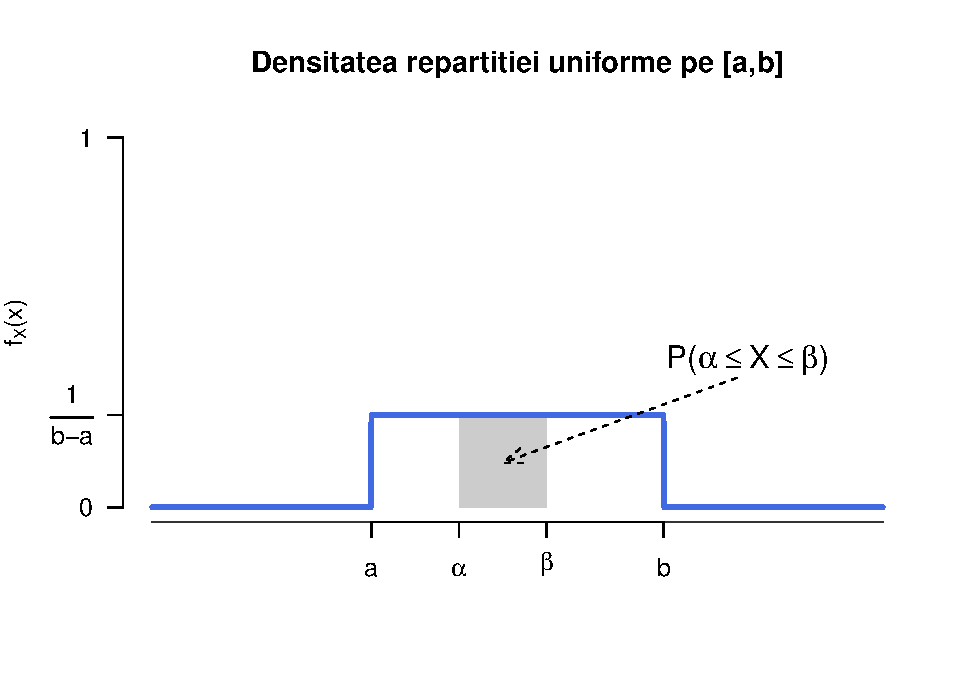
\includegraphics[width=0.7\linewidth]{Lab_6_files/figure-latex/unnamed-chunk-3-1} \end{center}

Funcția de repartiție a repartiției uniforme este

\[
  F_X(x) =\int_{-\infty}^{x}f_X(t)\,dt = \left\{\begin{array}{ll}
    0, & x\leq a\\
    \frac{x-a}{b-a}, & x\in(a,b)\\
    1, & x\geq b
  \end{array}\right.
\]

\begin{center}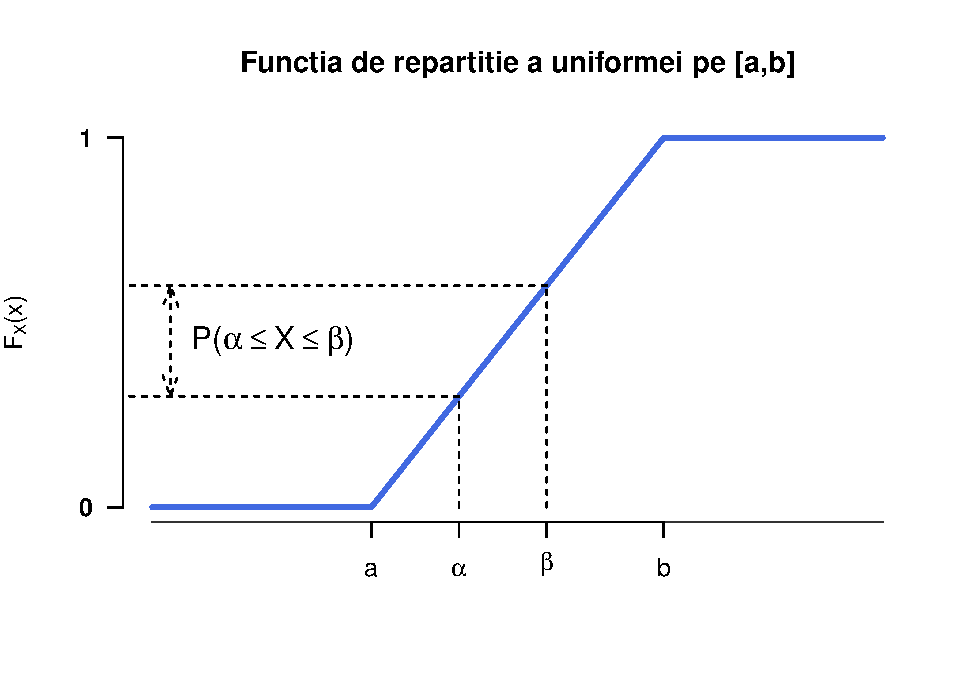
\includegraphics[width=0.7\linewidth]{Lab_6_files/figure-latex/unnamed-chunk-4-1} \end{center}

Media și varianța variabilei aleatoare \(X\) repartizate uniform pe
\([a,b]\) sunt egale cu

\[
  \mathbb{E}[X] = \frac{a+b}{2},\qquad Var(X) = \frac{(a-b)^2}{12}. 
\]

Variabilele aleatoare repartizate uniform joacă un rol important în
teoria simulării variabilelor aleatoare datorită următorului rezultat
datorat lui Paul Levy și numit \emph{teorema de universalitate a
repartiției uniforme}:

\begin{rmdinsight}
Fie \(X\) o variabilă aleatoare reală cu funcția de repartiție \(F\),
\(U\) o variabilă aleatoare repartizată uniform pe \([0,1]\) și fie
funcția \emph{cuantilă} (inversa generalizată) asociată lui \(F\),
\(F^{-1}:(0,1)\to\mathbb{R}\) definită prin

\[
  F^{-1}(u) = \inf\{x\in\mathbb{R}\,|\,F(x)\geq u\}, \quad \forall u\in(0,1).
\] Atunci \(X\) și \(F^{-1}(U)\) sunt repartizate la fel.
\end{rmdinsight}

În R putem să

\begin{itemize}
\tightlist
\item
  generăm observații independente din repartiția \(\mathcal{U}([a, b])\)
  (e.g. \(a = 3\) și \(b = 5\))
\end{itemize}

\begin{Shaded}
\begin{Highlighting}[]
\KeywordTok{runif}\NormalTok{(}\DecValTok{10}\NormalTok{, }\DecValTok{3}\NormalTok{, }\DecValTok{5}\NormalTok{)}
\NormalTok{ [}\DecValTok{1}\NormalTok{] }\FloatTok{4.433568} \FloatTok{3.481831} \FloatTok{4.223671} \FloatTok{3.865685} \FloatTok{4.287327} \FloatTok{3.929126} \FloatTok{3.041330}
\NormalTok{ [}\DecValTok{8}\NormalTok{] }\FloatTok{3.840754} \FloatTok{4.160534} \FloatTok{4.643392}
\end{Highlighting}
\end{Shaded}

\begin{itemize}
\tightlist
\item
  calculăm densitatea unei variabile aleatoare repartizate uniform pe
  \([a, b]\) în diferite puncte
\end{itemize}

\begin{Shaded}
\begin{Highlighting}[]
\KeywordTok{dunif}\NormalTok{(}\KeywordTok{c}\NormalTok{(}\FloatTok{3.1}\NormalTok{, }\FloatTok{3.7}\NormalTok{, }\FloatTok{3.95}\NormalTok{, }\FloatTok{4.86}\NormalTok{), }\DecValTok{3}\NormalTok{, }\DecValTok{5}\NormalTok{)}
\NormalTok{[}\DecValTok{1}\NormalTok{] }\FloatTok{0.5} \FloatTok{0.5} \FloatTok{0.5} \FloatTok{0.5}
\end{Highlighting}
\end{Shaded}

\begin{itemize}
\tightlist
\item
  calculăm funcția de repartiție a unei variabile repartizate uniform pe
  \([a,b]\) pentru diferite valori
\end{itemize}

\begin{Shaded}
\begin{Highlighting}[]
\KeywordTok{punif}\NormalTok{(}\KeywordTok{c}\NormalTok{(}\FloatTok{3.1}\NormalTok{, }\FloatTok{3.7}\NormalTok{, }\FloatTok{3.95}\NormalTok{, }\FloatTok{4.86}\NormalTok{), }\DecValTok{3}\NormalTok{, }\DecValTok{5}\NormalTok{)}
\NormalTok{[}\DecValTok{1}\NormalTok{] }\FloatTok{0.050} \FloatTok{0.350} \FloatTok{0.475} \FloatTok{0.930}
\end{Highlighting}
\end{Shaded}

\begin{rmdexercise}
Fie \(X\) o variabilă aleatoare repartizată uniform pe \([2,7]\).
Determinați:

\begin{enumerate}
\def\labelenumi{\alph{enumi})}
\tightlist
\item
  \(\mathbb{P}(X\in\{1,2,3,4,5,6,7\})\)
\item
  \(\mathbb{P}(X<3)\) și \(\mathbb{P}(X\leq 3)\)
\item
  \(\mathbb{P}(X\leq 3 \cup X>4)\)
\item
  Generați \(250\) de observații din repartiția dată, trasați histograma
  acestora și suprapuneți densitatea repartiției date (vezi figura de
  mai jos).
\end{enumerate}
\end{rmdexercise}

\begin{center}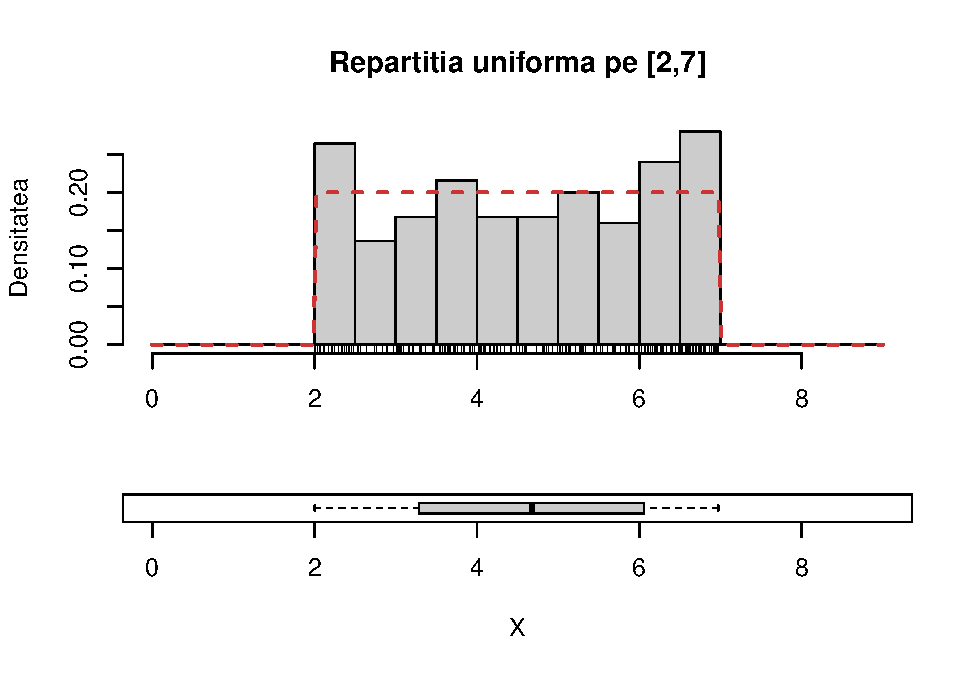
\includegraphics[width=0.7\linewidth]{Lab_6_files/figure-latex/unnamed-chunk-10-1} \end{center}

\begin{rmdexercise}
Dacă \(X\) o variabilă aleatoare repartizată uniform pe \([a,b]\) și
\([c,d]\subset [a,b]\) este un subinterval, atunci repartiția
condiționată a lui \(X\) la \(X\in [c,d]\) este \(\mathcal{U}[c,d]\).
\end{rmdexercise}

\section{Repartiția Normală}\label{repartitia-normala}

Spunem că o variabilă aleatoare \(X\) este repartizată \emph{normal} sau
\emph{Gaussian} de medie \(\mu\) și varianță \(\sigma^2\), și se notează
cu \(X\sim\mathcal{N}(\mu, \sigma^2)\), dacă densitatea ei are forma

\[
  f_X(x) \left(\overset{not}{=} \varphi(x)\right) = \frac{1}{\sqrt{2\pi}\sigma}e^{-\frac{(x-\mu)^2}{2\sigma^2}}, \quad x\in\mathbb{R}.
\]

\begin{center}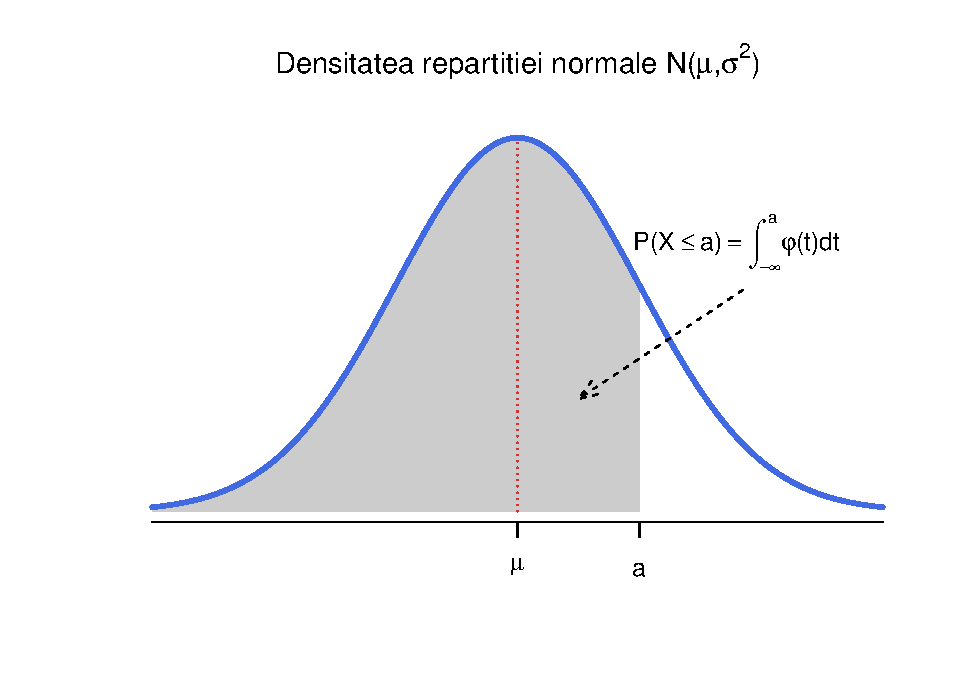
\includegraphics[width=0.7\linewidth]{Lab_6_files/figure-latex/unnamed-chunk-12-1} \end{center}

Funcția de repartiție a unei variabile
\(X\sim\mathcal{N}(\mu, \sigma^2)\) este dată de

\[
  F_X(x) \left(\overset{not}{=} \Phi(x)\right) = \int_{-\infty}^{x}\varphi(t)\,dt = \frac{1}{\sqrt{2\pi}\sigma}\int_{-\infty}^{x}e^{-\frac{(t-\mu)^2}{2\sigma^2}}\,dt.
\]

Pentru funcția de repartiție nu avem o formulă explicită de calcul, ea
poate fi aproximată cu ajutorul descompunerii în serie. În cazul
variabilelor \emph{normale standard} (\(X\sim\mathcal{N}(0,1)\)) avem
proprietățile

\begin{enumerate}
\def\labelenumi{\alph{enumi})}
\tightlist
\item
  \(\Phi(x) = 1-\Phi(-x)\) pentru toate valorile \(x\in\mathbb{R}\)
\item
  \(1-\Phi(a)\leq\frac{1}{2}e^{-\frac{a^2}{2}}\) pentru
  \(a>0\)\footnote{Pentru mai multe astfel de inegalități se poate
    consulta cartea (capitolul 2): Lin, Z. și Bai, Z. \emph{Probability
    Inequalities}, Springer, 2010.}
\end{enumerate}

\begin{center}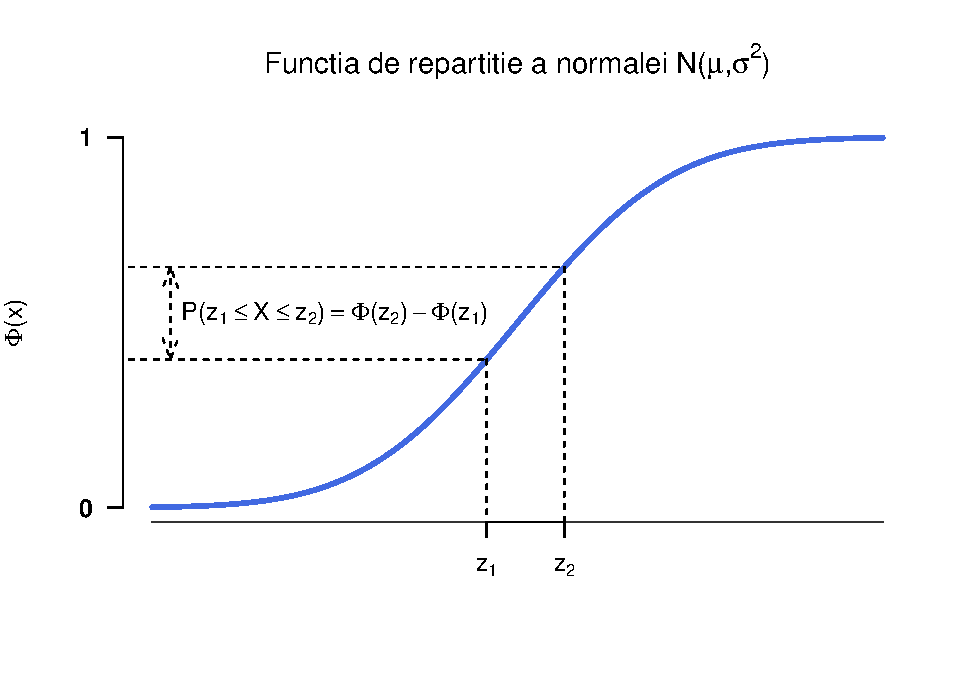
\includegraphics[width=0.7\linewidth]{Lab_6_files/figure-latex/unnamed-chunk-13-1} \end{center}

Media și varianța variabilei aleatoare \(X\) repartizate normal de
parametrii \(\mathcal{N}(\mu, \sigma^2)\) sunt egale cu

\[
  \mathbb{E}[X] = \mu,\quad Var(X) = \sigma^2. 
\] Mai mult, momentele de ordin se pot calcula cu ușurință și avem că

\[
  \mathbb{E}[X^k] = \left\{\begin{array}{ll}
      \sigma^k (k-1)!!, & \text{$k$ este par} \\
      0, & \text{$k$ este impar}.
  \end{array}\right.
\]

Pentru o variabilă aleatoare repartizată normal, avem următoarea regulă
numită și regula \(68-95-99.7\%\):

\begin{rmdinsight}
Fie \(X\) o variabilă aleatoare repartizată
\(\mathcal{N}(\mu, \sigma^2)\). Atunci

\begin{align*}
  \mathbb{P}(|X-\mu|<\sigma) &\approx 0.68\\
  \mathbb{P}(|X-\mu|<2\sigma) &\approx 0.95\\
  \mathbb{P}(|X-\mu|<3\sigma) &\approx 0.997
\end{align*}
\end{rmdinsight}

În R putem să

\begin{itemize}
\tightlist
\item
  generăm observații independente din repartiția
  \(\mathcal{N}(\mu, \sigma^2)\) (e.g. \(\mu = 0\) și \(\sigma^2 = 2\) -
  în R funcțiile \texttt{rnorm}, \texttt{dnorm}, \texttt{pnorm} și
  \texttt{qnorm} primesc ca parametrii media și abaterea standard,
  \(\sigma\) \textbf{nu} varianța \(\sigma^2\))
\end{itemize}

\begin{Shaded}
\begin{Highlighting}[]
\KeywordTok{rnorm}\NormalTok{(}\DecValTok{10}\NormalTok{, }\DataTypeTok{mean =} \DecValTok{0}\NormalTok{, }\DataTypeTok{sd =} \KeywordTok{sqrt}\NormalTok{(}\DecValTok{2}\NormalTok{))}
\NormalTok{ [}\DecValTok{1}\NormalTok{]  }\FloatTok{2.11174310}  \FloatTok{2.58674379} \OperatorTok{-}\FloatTok{2.18307577}  \FloatTok{0.51710533}  \FloatTok{0.16850263}
\NormalTok{ [}\DecValTok{6}\NormalTok{]  }\FloatTok{0.09291647}  \FloatTok{0.43628036}  \FloatTok{0.86380483} \OperatorTok{-}\FloatTok{1.96630543}  \FloatTok{0.30378068}
\end{Highlighting}
\end{Shaded}

\begin{itemize}
\tightlist
\item
  calculăm densitatea unei variabile aleatoare repartizate normal
  \(\mathcal{N}(\mu, \sigma^2)\) în diferite puncte
\end{itemize}

\begin{Shaded}
\begin{Highlighting}[]
\KeywordTok{dnorm}\NormalTok{(}\KeywordTok{seq}\NormalTok{(}\OperatorTok{-}\DecValTok{2}\NormalTok{, }\DecValTok{2}\NormalTok{, }\DataTypeTok{length.out =} \DecValTok{15}\NormalTok{), }\DataTypeTok{mean =} \DecValTok{3}\NormalTok{, }\DataTypeTok{sd =} \DecValTok{5}\NormalTok{)}
\NormalTok{ [}\DecValTok{1}\NormalTok{] }\FloatTok{0.04839414} \FloatTok{0.05115647} \FloatTok{0.05390019} \FloatTok{0.05660592} \FloatTok{0.05925368} \FloatTok{0.06182308}
\NormalTok{ [}\DecValTok{7}\NormalTok{] }\FloatTok{0.06429362} \FloatTok{0.06664492} \FloatTok{0.06885700} \FloatTok{0.07091058} \FloatTok{0.07278734} \FloatTok{0.07447021}
\NormalTok{[}\DecValTok{13}\NormalTok{] }\FloatTok{0.07594361} \FloatTok{0.07719368} \FloatTok{0.07820854}
\end{Highlighting}
\end{Shaded}

\begin{itemize}
\tightlist
\item
  calculăm funcția de repartiție a unei variabile repartizate normal
  \(\mathcal{N}(\mu, \sigma^2)\) pentru diferite valori
\end{itemize}

\begin{Shaded}
\begin{Highlighting}[]
\KeywordTok{pnorm}\NormalTok{(}\KeywordTok{seq}\NormalTok{(}\OperatorTok{-}\DecValTok{1}\NormalTok{, }\DecValTok{1}\NormalTok{, }\DataTypeTok{length.out =} \DecValTok{15}\NormalTok{), }\DataTypeTok{mean =} \DecValTok{3}\NormalTok{, }\DataTypeTok{sd =} \DecValTok{1}\NormalTok{)}
\NormalTok{ [}\DecValTok{1}\NormalTok{] }\FloatTok{3.167124e-05} \FloatTok{5.736006e-05} \FloatTok{1.018892e-04} \FloatTok{1.775197e-04} \FloatTok{3.033834e-04}
\NormalTok{ [}\DecValTok{6}\NormalTok{] }\FloatTok{5.086207e-04} \FloatTok{8.365374e-04} \FloatTok{1.349898e-03} \FloatTok{2.137367e-03} \FloatTok{3.320943e-03}
\NormalTok{[}\DecValTok{11}\NormalTok{] }\FloatTok{5.063995e-03} \FloatTok{7.579219e-03} \FloatTok{1.113549e-02} \FloatTok{1.606229e-02} \FloatTok{2.275013e-02}
\end{Highlighting}
\end{Shaded}

\begin{itemize}
\tightlist
\item
  calculăm cuantilele de ordin \(\alpha\in(0,1)\) (i.e.~valoarea
  \(z_{\alpha}\) pentru care \(\Phi(z_{\alpha}) = \alpha\) sau altfel
  spus \(z_{\alpha} = \Phi^{-1}(\alpha)\))
\end{itemize}

\begin{Shaded}
\begin{Highlighting}[]
\KeywordTok{qnorm}\NormalTok{(}\KeywordTok{c}\NormalTok{(}\FloatTok{0.01}\NormalTok{, }\FloatTok{0.025}\NormalTok{, }\FloatTok{0.05}\NormalTok{, }\FloatTok{0.25}\NormalTok{, }\FloatTok{0.5}\NormalTok{, }\FloatTok{0.75}\NormalTok{, }\FloatTok{0.95}\NormalTok{, }\FloatTok{0.975}\NormalTok{, }\FloatTok{0.99}\NormalTok{), }\DataTypeTok{mean =} \DecValTok{0}\NormalTok{, }\DataTypeTok{sd =} \DecValTok{1}\NormalTok{)}
\NormalTok{[}\DecValTok{1}\NormalTok{] }\OperatorTok{-}\FloatTok{2.3263479} \OperatorTok{-}\FloatTok{1.9599640} \OperatorTok{-}\FloatTok{1.6448536} \OperatorTok{-}\FloatTok{0.6744898}  \FloatTok{0.0000000}  \FloatTok{0.6744898}
\NormalTok{[}\DecValTok{7}\NormalTok{]  }\FloatTok{1.6448536}  \FloatTok{1.9599640}  \FloatTok{2.3263479}
\end{Highlighting}
\end{Shaded}

\begin{rmdexercise}
Fie \(X\) o variabilă aleatoare repartizată
\(\mathcal{N}(\mu, \sigma^2)\). Atunci pentru \(\mu = 1\) și
\(\sigma = 3\) calculați:

\begin{enumerate}
\def\labelenumi{\arabic{enumi})}
\tightlist
\item
  \(\mathbb{P}(\text{$X$ este par})\)
\item
  \(\mathbb{P}(X<3.4)\) și \(\mathbb{P}(X>1.3)\)
\item
  \(\mathbb{P}(1<X<4)\)
\item
  \(\mathbb{P}(X\in [2,3]\cup[3.5,5])\)
\item
  \(\mathbb{P}(|X-3|>6)\)
\end{enumerate}
\end{rmdexercise}

\begin{rmdexercise}
Fie \(X\) o variabilă aleatoare repartizată
\(\mathcal{N}(\mu, \sigma^2)\). Pentru \(\mu = 0\) și
\(\sigma^2 \in \{0.2, 0.5, 1.5, 5\}\) trasați pe același grafic
densitățile repartițiilor normale cu parametrii
\(\mathcal{N}(\mu, \sigma^2)\). Adăugați legendele corespunzătoare.
Aceeași cerință pentru funcțiile de repartiție.
\end{rmdexercise}

\begin{center}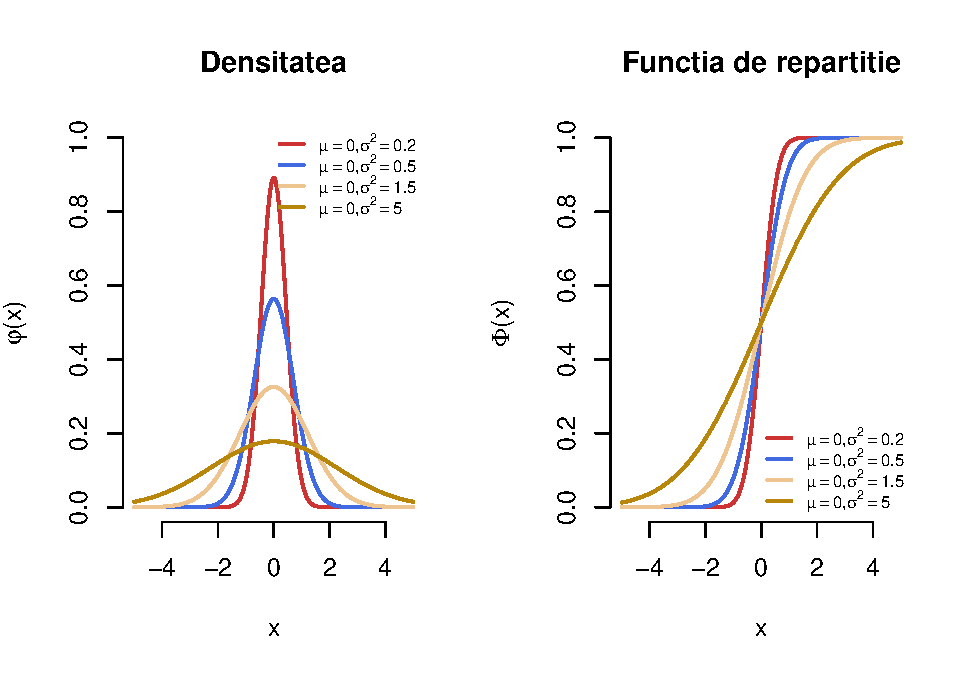
\includegraphics[width=0.7\linewidth]{Lab_6_files/figure-latex/unnamed-chunk-21-1} \end{center}

\begin{rmdexercise}
Generați \(250\) de observații din repartiția \(\mathcal{N}(0, 2)\),
trasați histograma acestora și suprapuneți densitatea repartiției date
(vezi figura de mai jos).
\end{rmdexercise}

\begin{center}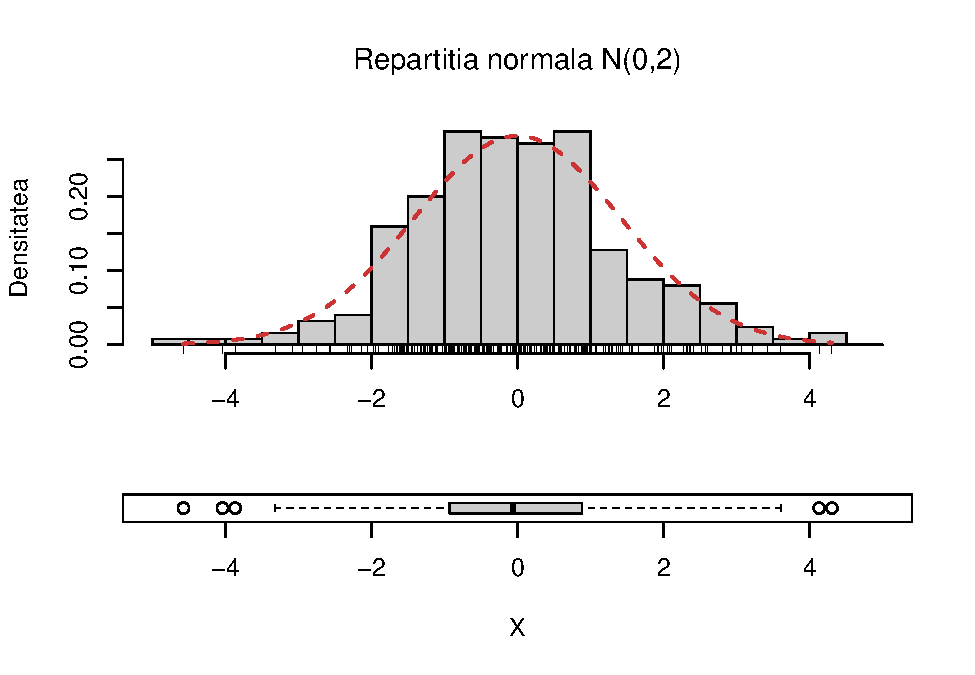
\includegraphics[width=0.7\linewidth]{Lab_6_files/figure-latex/unnamed-chunk-23-1} \end{center}

\begin{rmdexercise}
Fie \(X\) o variabilă aleatoare repartizată normal de parametrii \(\mu\)
și \(\sigma^2\). Ilustrați grafic pentru \(\mu = 0\) și \(\sigma = 1\)
că are loc următoarea inegalitate:

\[
  \left(\frac{1}{x}-\frac{1}{x^3}\right)\phi(x)<1-\Phi(x)<\frac{1}{x}\phi(x), \quad x>0.
\]
\end{rmdexercise}

\begin{center}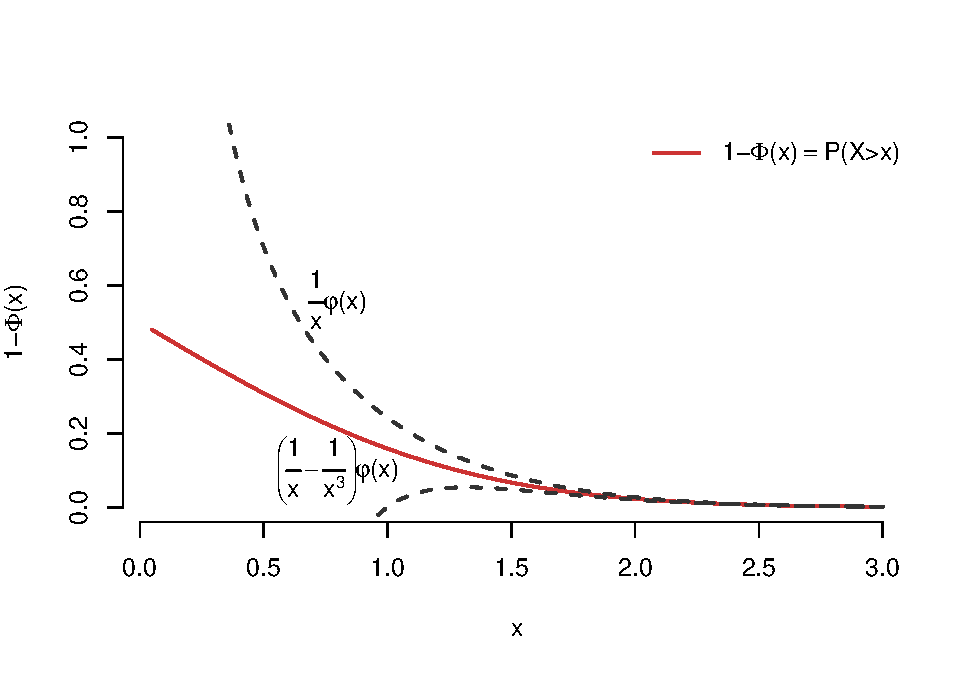
\includegraphics[width=0.7\linewidth]{Lab_6_files/figure-latex/unnamed-chunk-25-1} \end{center}

\section{Repartiția Log-Normală}\label{repartitia-log-normala}

Spune că o variabilă aleatoare \(X\) este repartizată log-normal de
parametrii \(\mu\) și \(\sigma^2\), și notăm
\(X\sim LN(\mu, \sigma^2)\), dacă \(\ln(X)\) este repartizată normal de
parametrii \(\mu\) și \(\sigma^2\). Cu alte cuvinte dacă
\(Y\sim \mathcal{N}(\mu, \sigma^2)\) atunci
\(X=e^Y\sim LN(\mu, \sigma^2)\). Densitatea repartiției log-normale
\(LN(\mu, \sigma^2)\) este

\[
    f_X(x) = \frac{1}{x\sigma\sqrt{2\pi}}e^{-\frac{(\ln(x)-\mu)^2}{2\sigma^2}}, \quad x\in (0, +\infty).
\]

\begin{center}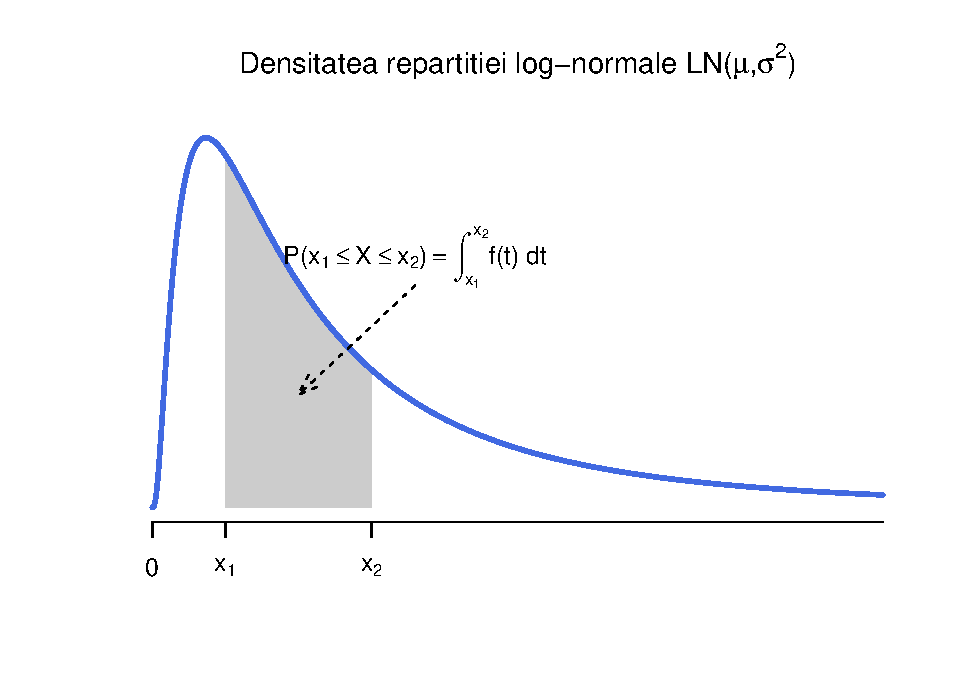
\includegraphics[width=0.7\linewidth]{Lab_6_files/figure-latex/unnamed-chunk-26-1} \end{center}

Funcția de repartiție a unei variabile aleatoare
\(X\sim LN(\mu, \sigma^2)\) este dată de

\[
  F_{X}(x) = \int_{-\infty}^{x}f_X(t)\,dt = \frac{1}{\sqrt{2\pi}\sigma}\int_{-\infty}^{x}\frac{1}{t}e^{-\frac{(\ln(t)-\mu)^2}{2\sigma^2}}\,dt
\]

și, ca și în cazul repartiției normale, nu are o formulă explicită de
calcul.

\begin{center}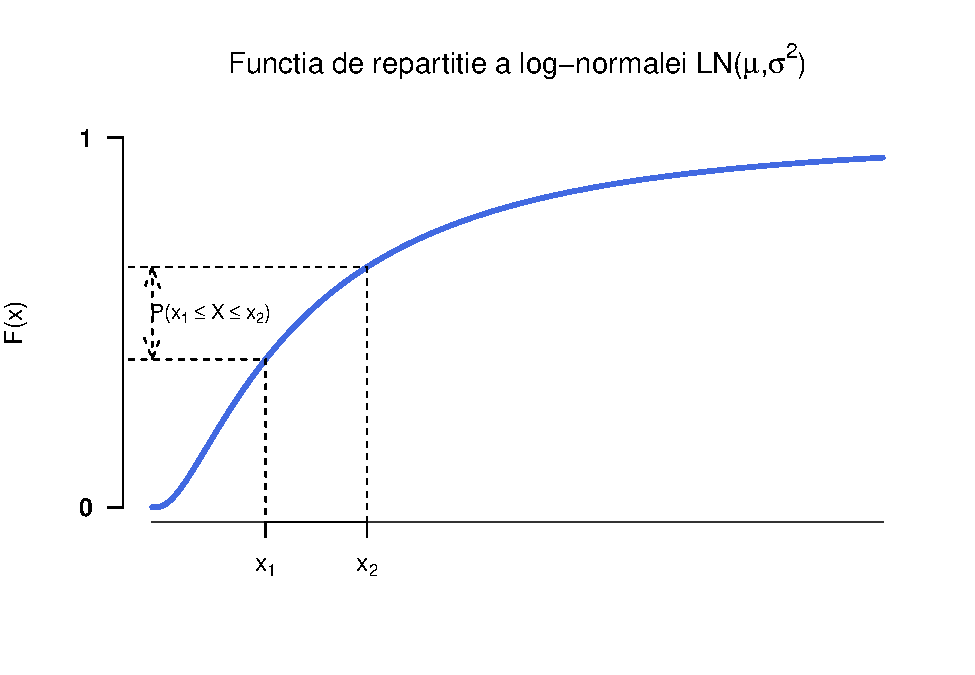
\includegraphics[width=0.7\linewidth]{Lab_6_files/figure-latex/unnamed-chunk-27-1} \end{center}

Media și varianța variabilei aleatoare \(X\) repartizate log-normal de
parametrii \(LN(\mu, \sigma^2)\) sunt egale cu

\[
  \mathbb{E}[X] = e^{\mu+\frac{\sigma^2}{2}},\quad Var(X) = \left(e^{\sigma^2}-1\right)e^{2\mu+\sigma^2}. 
\]

\begin{rmdexercise}
Arătați că media și varianța unei variabile aleatoare repartizate
log-normal de parametrii \(\mu\) și \(\sigma^2\) sunt egale cu

\[
  \mathbb{E}[X] = e^{\mu+\frac{\sigma^2}{2}},\quad Var(X) = \left(e^{\sigma^2}-1\right)e^{2\mu+\sigma^2}. 
\]
\end{rmdexercise}

În R putem să

\begin{itemize}
\tightlist
\item
  generăm observații independente din repartiția \(LN(\mu, \sigma^2)\)
  (e.g. \(\mu = 0\) și \(\sigma^2 = 3\) - ca și în cazul repartiției
  normale, funcțiile \texttt{rlnorm}, \texttt{dlnorm}, \texttt{plnorm}
  și \texttt{qlnorm} primesc ca parametrii media și abaterea standard,
  \(\sigma\) pentru \(\ln(X)\) - variabila normală)
\end{itemize}

\begin{Shaded}
\begin{Highlighting}[]
\KeywordTok{rlnorm}\NormalTok{(}\DecValTok{15}\NormalTok{, }\DataTypeTok{meanlog =} \DecValTok{0}\NormalTok{, }\DataTypeTok{sdlog =} \KeywordTok{sqrt}\NormalTok{(}\DecValTok{3}\NormalTok{))}
\NormalTok{ [}\DecValTok{1}\NormalTok{]  }\FloatTok{2.13141475}  \FloatTok{6.27258447}  \FloatTok{2.18850080}  \FloatTok{3.15407005}  \FloatTok{0.13970018}
\NormalTok{ [}\DecValTok{6}\NormalTok{]  }\FloatTok{0.52638598} \FloatTok{12.91237780}  \FloatTok{0.12004802}  \FloatTok{1.56359485}  \FloatTok{2.01674623}
\NormalTok{[}\DecValTok{11}\NormalTok{]  }\FloatTok{5.42024453}  \FloatTok{0.54647199}  \FloatTok{1.31619806}  \FloatTok{0.04716763}  \FloatTok{1.79762358}
\end{Highlighting}
\end{Shaded}

\begin{itemize}
\tightlist
\item
  calculăm densitatea unei variabile aleatoare repartizate log-normal
  \(LN(\mu, \sigma^2)\) în diferite puncte
\end{itemize}

\begin{Shaded}
\begin{Highlighting}[]
\KeywordTok{dlnorm}\NormalTok{(}\KeywordTok{seq}\NormalTok{(}\DecValTok{0}\NormalTok{, }\DecValTok{5}\NormalTok{, }\DataTypeTok{length.out =} \DecValTok{20}\NormalTok{), }\DataTypeTok{meanlog =} \DecValTok{3}\NormalTok{, }\DataTypeTok{sdlog =} \DecValTok{5}\NormalTok{)}
\NormalTok{ [}\DecValTok{1}\NormalTok{] }\FloatTok{0.00000000} \FloatTok{0.20820751} \FloatTok{0.11627647} \FloatTok{0.08196427} \FloatTok{0.06370023} \FloatTok{0.05226715}
\NormalTok{ [}\DecValTok{7}\NormalTok{] }\FloatTok{0.04440086} \FloatTok{0.03864103} \FloatTok{0.03423291} \FloatTok{0.03074580} \FloatTok{0.02791546} \FloatTok{0.02557044}
\NormalTok{[}\DecValTok{13}\NormalTok{] }\FloatTok{0.02359456} \FloatTok{0.02190618} \FloatTok{0.02044622} \FloatTok{0.01917084} \FloatTok{0.01804680} \FloatTok{0.01704845}
\NormalTok{[}\DecValTok{19}\NormalTok{] }\FloatTok{0.01615564} \FloatTok{0.01535234}
\end{Highlighting}
\end{Shaded}

\begin{itemize}
\tightlist
\item
  calculăm funcția de repartiție a unei variabile repartizate log-normal
  \(LN(\mu, \sigma^2)\) pentru diferite valori
\end{itemize}

\begin{Shaded}
\begin{Highlighting}[]
\KeywordTok{plnorm}\NormalTok{(}\KeywordTok{seq}\NormalTok{(}\DecValTok{0}\NormalTok{, }\DecValTok{15}\NormalTok{, }\DataTypeTok{length.out =} \DecValTok{25}\NormalTok{), }\DataTypeTok{meanlog =} \DecValTok{3}\NormalTok{, }\DataTypeTok{sdlog =} \DecValTok{1}\NormalTok{)}
\NormalTok{ [}\DecValTok{1}\NormalTok{] }\FloatTok{0.0000000000} \FloatTok{0.0002602257} \FloatTok{0.0027443707} \FloatTok{0.0088606283} \FloatTok{0.0185933103}
\NormalTok{ [}\DecValTok{6}\NormalTok{] }\FloatTok{0.0314027650} \FloatTok{0.0466497221} \FloatTok{0.0637426806} \FloatTok{0.0821791298} \FloatTok{0.1015482283}
\NormalTok{[}\DecValTok{11}\NormalTok{] }\FloatTok{0.1215206945} \FloatTok{0.1418356830} \FloatTok{0.1622882185} \FloatTok{0.1827183180} \FloatTok{0.2030019832}
\NormalTok{[}\DecValTok{16}\NormalTok{] }\FloatTok{0.2230439002} \FloatTok{0.2427715876} \FloatTok{0.2621307274} \FloatTok{0.2810814477} \FloatTok{0.2995953616}
\NormalTok{[}\DecValTok{21}\NormalTok{] }\FloatTok{0.3176532076} \FloatTok{0.3352429649} \FloatTok{0.3523583472} \FloatTok{0.3689975944} \FloatTok{0.3851625036}
\end{Highlighting}
\end{Shaded}

\begin{itemize}
\tightlist
\item
  calculăm cuantilele de ordin \(\alpha\in(0,1)\)
\end{itemize}

\begin{Shaded}
\begin{Highlighting}[]
\KeywordTok{qlnorm}\NormalTok{(}\KeywordTok{c}\NormalTok{(}\FloatTok{0.01}\NormalTok{, }\FloatTok{0.025}\NormalTok{, }\FloatTok{0.05}\NormalTok{, }\FloatTok{0.25}\NormalTok{, }\FloatTok{0.5}\NormalTok{, }\FloatTok{0.75}\NormalTok{, }\FloatTok{0.95}\NormalTok{, }\FloatTok{0.975}\NormalTok{, }\FloatTok{0.99}\NormalTok{), }\DataTypeTok{meanlog =} \DecValTok{0}\NormalTok{, }\DataTypeTok{sdlog =} \DecValTok{1}\NormalTok{)}
\NormalTok{[}\DecValTok{1}\NormalTok{]  }\FloatTok{0.09765173}  \FloatTok{0.14086349}  \FloatTok{0.19304082}  \FloatTok{0.50941628}  \FloatTok{1.00000000}  \FloatTok{1.96303108}
\NormalTok{[}\DecValTok{7}\NormalTok{]  }\FloatTok{5.18025160}  \FloatTok{7.09907138} \FloatTok{10.24047366}
\end{Highlighting}
\end{Shaded}

\begin{rmdexercise}
Fie \(X\) o variabilă aleatoare repartizată \(LN(\mu, \sigma^2)\).
Pentru \(\mu = 0\) și \(\sigma \in \{0.25, 0.5, 1.5, 5\}\) trasați pe
același grafic densitățile repartițiilor log-normale cu parametrii
\(LN(\mu, \sigma^2)\). Adăugați legendele corespunzătoare. Aceeași
cerință pentru funcțiile de repartiție.
\end{rmdexercise}

\begin{center}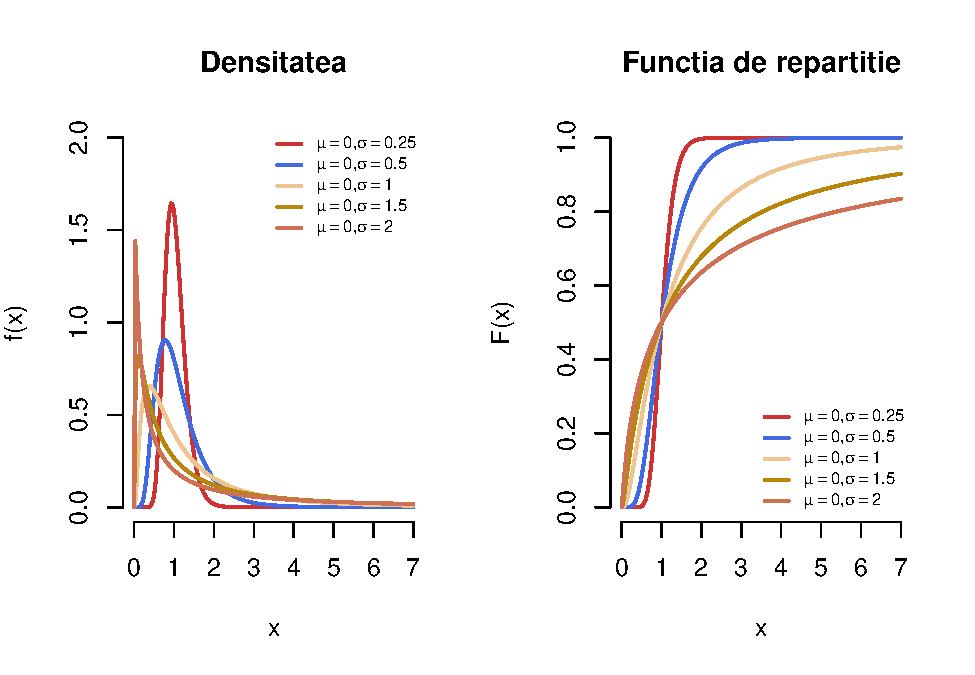
\includegraphics[width=0.7\linewidth]{Lab_6_files/figure-latex/unnamed-chunk-34-1} \end{center}

\begin{rmdexercise}
Generați \(500\) de observații din repartiția \(LN(0, 2)\), trasați
histograma acestora și suprapuneți densitatea repartiției date (vezi
figura de mai jos).
\end{rmdexercise}

\begin{center}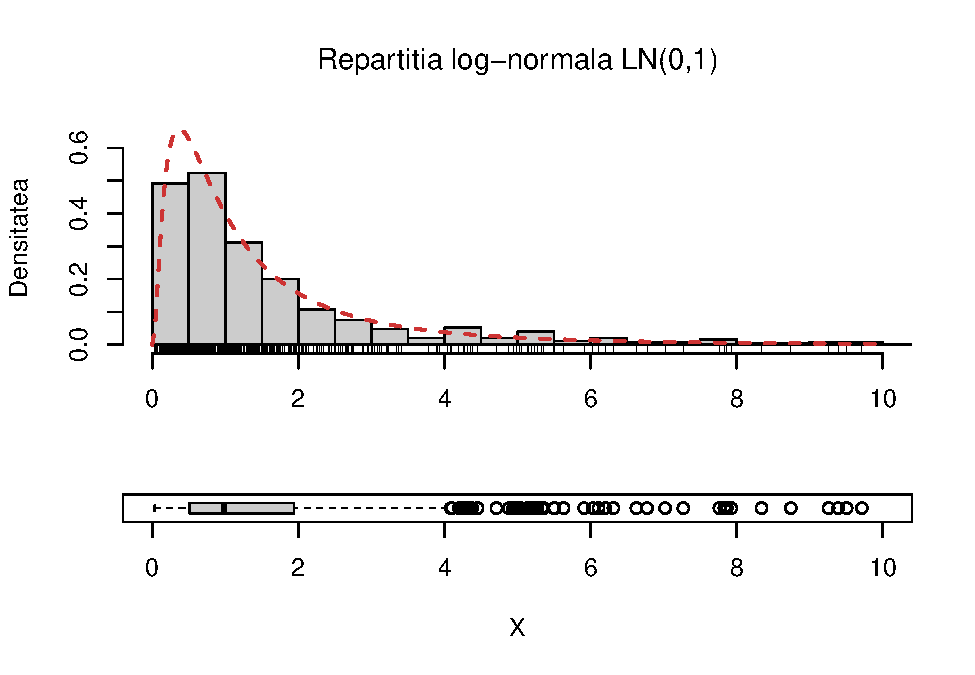
\includegraphics[width=0.7\linewidth]{Lab_6_files/figure-latex/unnamed-chunk-36-1} \end{center}

Printre fenomenele care pot fi modelate cu ajutorul repartiției
log-normale se numără: cantitatea de lapte produsă de vaci, cantitatea
de ploaie dintr-o perioadă dată, repartiția mărimii picăturilor de
ploaie, volumul de gaz dintr-o rezervă petrolieră, etc. Pentru mai multe
aplicații se poate consulta lucrarea lui Limpert, E., Stajel, W. și
Abbt, M.
\href{http://stat.ethz.ch/~stahel/lognormal/bioscience.pdf}{Log-normal
Distributions across the Sciences: Keys and Clues}, \emph{BioScience},
Vol. 51, Nr. 5, 2001.

\section{Repartiția Exponențială}\label{repartitia-exponentiala}

Spunem că o variabilă aleatoare \(X\) este repartizată
\emph{exponențial} de parametru \(\lambda\), și se notează cu
\(X\sim\mathcal{E}(\lambda)\), dacă densitatea ei are forma

\[
  f_X(x) = \lambda e^{-\lambda x}\mathbb{1}_{\mathbb{R}_+}(x),\quad \forall x\in\mathbb{R}.
\]

\begin{center}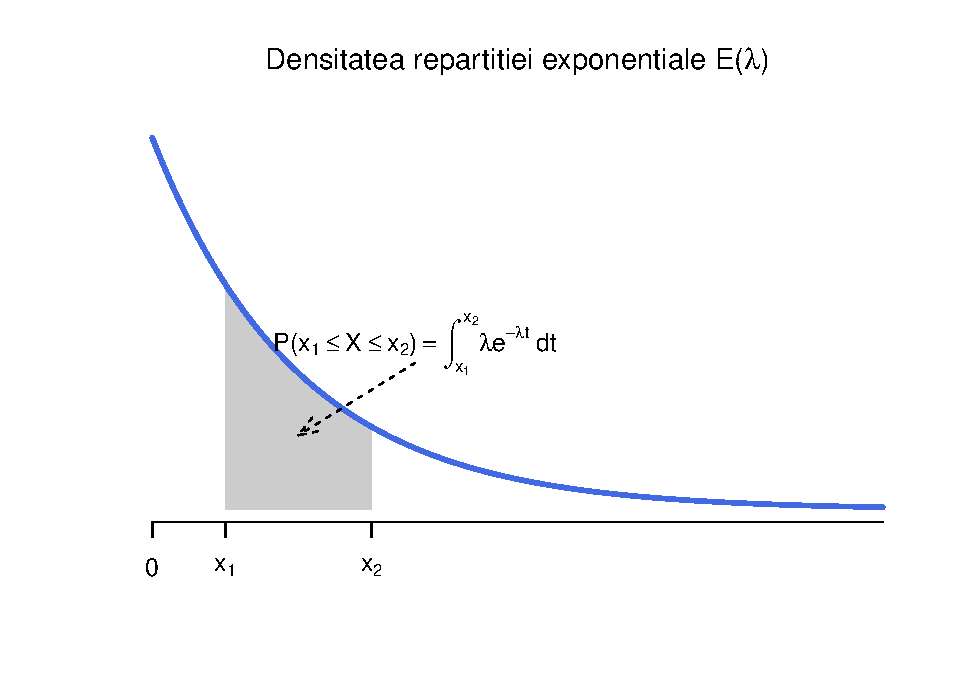
\includegraphics[width=0.7\linewidth]{Lab_6_files/figure-latex/unnamed-chunk-37-1} \end{center}

Funcția de repartiție a unei variabile aleatoare
\(X\sim \mathcal{E}(\lambda)\) este dată de

\[
  F_{X}(x) = 1 - e^{-\lambda x}\mathbb{1}_{\mathbb{R}_+}(x), \quad x\in \mathbb{R}.
\]

\begin{center}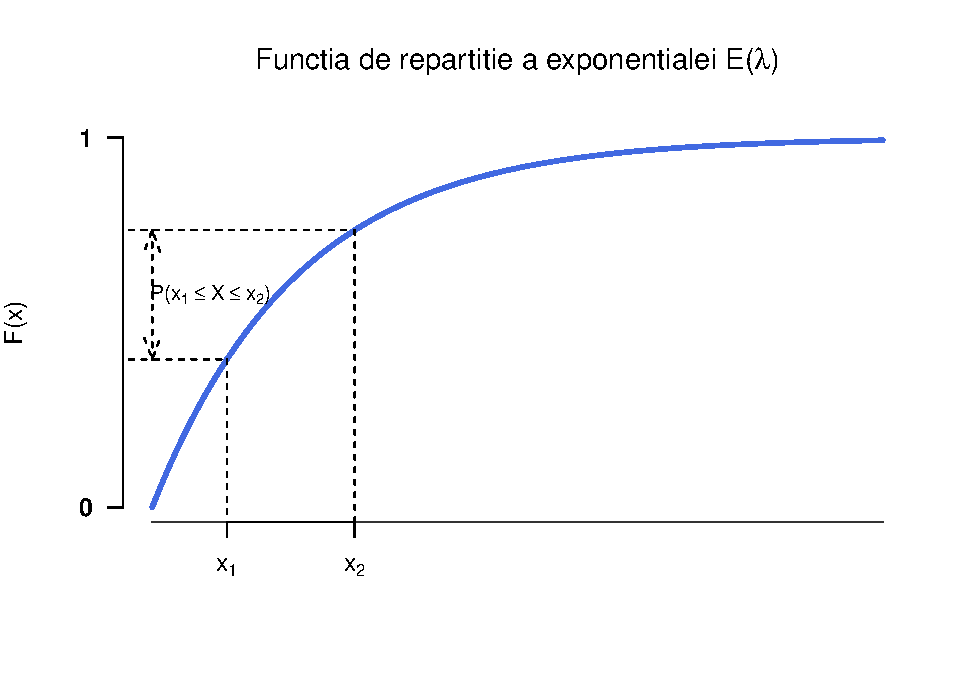
\includegraphics[width=0.7\linewidth]{Lab_6_files/figure-latex/unnamed-chunk-38-1} \end{center}

Media și varianța variabilei aleatoare \(X\) repartizate exponențial de
parametru \(\lambda\) sunt egale cu

\[
  \mathbb{E}[X] = \frac{1}{\lambda},\quad Var(X) =  \frac{1}{\lambda^2}. 
\]

\begin{rmdexercise}
Arătați că momentul de ordin \(k\), \(k\geq 1\), al unei variabile
aleatoare repartizate exponențial \(X\sim\mathcal{E}(\lambda)\) este
egal cu

\[
  \mathbb{E}[X^k] = \frac{k!}{\lambda^k}. 
\]
\end{rmdexercise}

\begin{rmdinsight}
Fie \(X\) o variabilă repartizată exponențial de parametru \(\lambda\).
Atunci are loc următoarea proprietate numită și \emph{lipsa de memorie}:

\[
      \mathbb{P}(X>s+t|X>s) = \mathbb{P}(X>t),\quad \forall s,t \geq 0. 
\]

Mai mult, dacă o variabilă aleatoare continuă\footnote{Pentru cazul
  discret avem variabila repartizată Geometric.} \(X\) verifică
proprietatea de mai sus atunci ea este repartizată exponențial.
\end{rmdinsight}

Variabilele aleatoare repartizate exponențial sunt utilizate în
modelarea fenomenelor care se desfășoară în timp continuu și care
satisfac (aproximativ) proprietatea lipsei de memorie: de exemplu timpul
de așteptare la un ghișeu, durata de viață a unui bec sau timpul până la
următoarea convorbire telefonică.

În R putem să

\begin{itemize}
\tightlist
\item
  generăm observații independente din repartiția
  \(\mathcal{E}(\lambda)\) (e.g. \(\lambda = 5\))
\end{itemize}

\begin{Shaded}
\begin{Highlighting}[]
\KeywordTok{rexp}\NormalTok{(}\DecValTok{15}\NormalTok{, }\DataTypeTok{rate =} \DecValTok{5}\NormalTok{)}
\NormalTok{ [}\DecValTok{1}\NormalTok{] }\FloatTok{0.13505357} \FloatTok{0.15392539} \FloatTok{0.25036131} \FloatTok{0.15351051} \FloatTok{0.00878456} \FloatTok{0.07362396}
\NormalTok{ [}\DecValTok{7}\NormalTok{] }\FloatTok{0.07543271} \FloatTok{0.18981181} \FloatTok{0.05540771} \FloatTok{0.05649451} \FloatTok{0.15878039} \FloatTok{0.39847262}
\NormalTok{[}\DecValTok{13}\NormalTok{] }\FloatTok{0.05191221} \FloatTok{0.07776034} \FloatTok{0.22483594}
\end{Highlighting}
\end{Shaded}

\begin{itemize}
\tightlist
\item
  calculăm densitatea unei variabile aleatoare repartizate exponențial
  \(\mathcal{E}(\lambda)\) în diferite puncte
\end{itemize}

\begin{Shaded}
\begin{Highlighting}[]
\KeywordTok{dexp}\NormalTok{(}\KeywordTok{seq}\NormalTok{(}\DecValTok{0}\NormalTok{, }\DecValTok{5}\NormalTok{, }\DataTypeTok{length.out =} \DecValTok{20}\NormalTok{), }\DataTypeTok{rate =} \DecValTok{5}\NormalTok{)}
\NormalTok{ [}\DecValTok{1}\NormalTok{] }\FloatTok{5.000000e+00} \FloatTok{1.341312e+00} \FloatTok{3.598237e-01} \FloatTok{9.652719e-02} \FloatTok{2.589462e-02}
\NormalTok{ [}\DecValTok{6}\NormalTok{] }\FloatTok{6.946555e-03} \FloatTok{1.863500e-03} \FloatTok{4.999070e-04} \FloatTok{1.341063e-04} \FloatTok{3.597568e-05}
\NormalTok{[}\DecValTok{11}\NormalTok{] }\FloatTok{9.650925e-06} \FloatTok{2.588981e-06} \FloatTok{6.945263e-07} \FloatTok{1.863153e-07} \FloatTok{4.998141e-08}
\NormalTok{[}\DecValTok{16}\NormalTok{] }\FloatTok{1.340814e-08} \FloatTok{3.596899e-09} \FloatTok{9.649130e-10} \FloatTok{2.588499e-10} \FloatTok{6.943972e-11}
\end{Highlighting}
\end{Shaded}

\begin{itemize}
\tightlist
\item
  calculăm funcția de repartiție a unei variabile repartizate
  exponențial \(\mathcal{E}(\lambda)\) pentru diferite valori
\end{itemize}

\begin{Shaded}
\begin{Highlighting}[]
\KeywordTok{pexp}\NormalTok{(}\KeywordTok{seq}\NormalTok{(}\DecValTok{0}\NormalTok{, }\DecValTok{5}\NormalTok{, }\DataTypeTok{length.out =} \DecValTok{15}\NormalTok{), }\DataTypeTok{rate =} \DecValTok{5}\NormalTok{)}
\NormalTok{ [}\DecValTok{1}\NormalTok{] }\FloatTok{0.0000000} \FloatTok{0.8323228} \FloatTok{0.9718843} \FloatTok{0.9952856} \FloatTok{0.9992095} \FloatTok{0.9998675} \FloatTok{0.9999778}
\NormalTok{ [}\DecValTok{8}\NormalTok{] }\FloatTok{0.9999963} \FloatTok{0.9999994} \FloatTok{0.9999999} \FloatTok{1.0000000} \FloatTok{1.0000000} \FloatTok{1.0000000} \FloatTok{1.0000000}
\NormalTok{[}\DecValTok{15}\NormalTok{] }\FloatTok{1.0000000}
\end{Highlighting}
\end{Shaded}

\begin{itemize}
\tightlist
\item
  calculăm cuantilele de ordin \(\alpha\in(0,1)\)
\end{itemize}

\begin{Shaded}
\begin{Highlighting}[]
\KeywordTok{qexp}\NormalTok{(}\KeywordTok{c}\NormalTok{(}\FloatTok{0.01}\NormalTok{, }\FloatTok{0.025}\NormalTok{, }\FloatTok{0.05}\NormalTok{, }\FloatTok{0.25}\NormalTok{, }\FloatTok{0.5}\NormalTok{, }\FloatTok{0.75}\NormalTok{, }\FloatTok{0.95}\NormalTok{, }\FloatTok{0.975}\NormalTok{, }\FloatTok{0.99}\NormalTok{), }\DataTypeTok{rate =} \DecValTok{5}\NormalTok{)}
\NormalTok{[}\DecValTok{1}\NormalTok{] }\FloatTok{0.002010067} \FloatTok{0.005063562} \FloatTok{0.010258659} \FloatTok{0.057536414} \FloatTok{0.138629436} \FloatTok{0.277258872}
\NormalTok{[}\DecValTok{7}\NormalTok{] }\FloatTok{0.599146455} \FloatTok{0.737775891} \FloatTok{0.921034037}
\end{Highlighting}
\end{Shaded}

\begin{rmdexercise}
Fie \(X\) o variabilă aleatoare repartizată \(\mathcal{E}(\lambda)\).
Pentru \(\lambda \in \{0.5, 1.5, 5\}\) trasați pe același grafic
densitățile repartițiilor exponențiale de parametru \(\lambda\).
Adăugați legendele corespunzătoare. Aceeași cerință pentru funcțiile de
repartiție.
\end{rmdexercise}

\begin{center}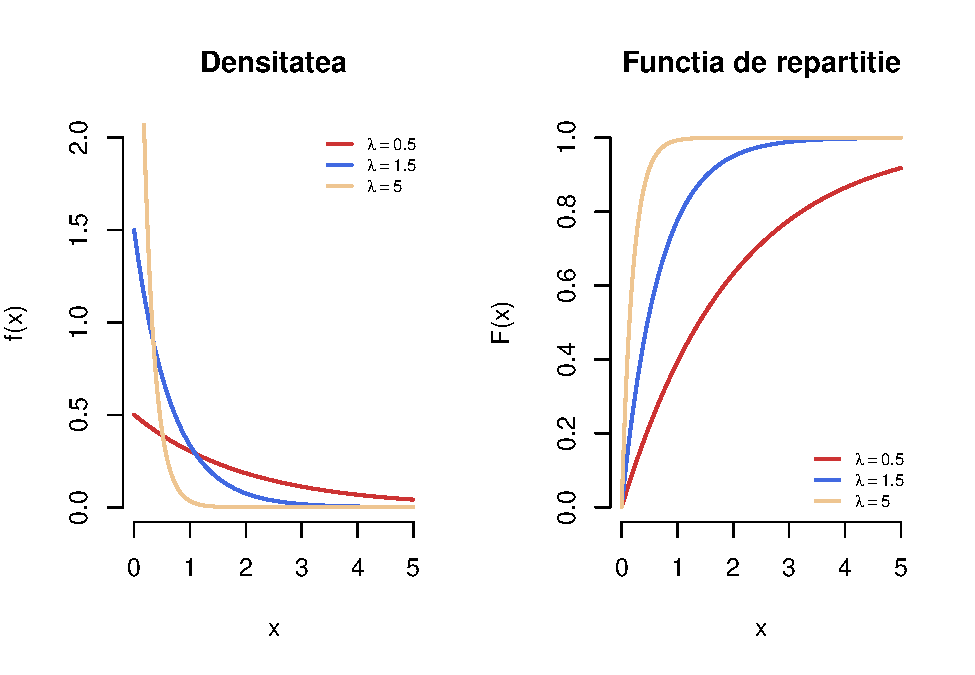
\includegraphics[width=0.7\linewidth]{Lab_6_files/figure-latex/unnamed-chunk-46-1} \end{center}

\begin{rmdexercise}
Folosind rezultatul de universalitate de la repartiția uniformă,
descrieți o procedură prin care puteți simula o variabilă aleatoare
repartizată exponențial \(\mathcal{E}(\lambda)\) și construiți o funcție
care permite generarea de \(n\) observații independente dintr-o
variabilă repartizată \(X\sim \mathcal{E}(\lambda)\).
\end{rmdexercise}

\begin{rmdexercise}
Generați \(250\) de observații din repartiția \(\mathcal{E}(3)\),
trasați histograma acestora și suprapuneți densitatea repartiției date
(vezi figura de mai jos).
\end{rmdexercise}

\begin{center}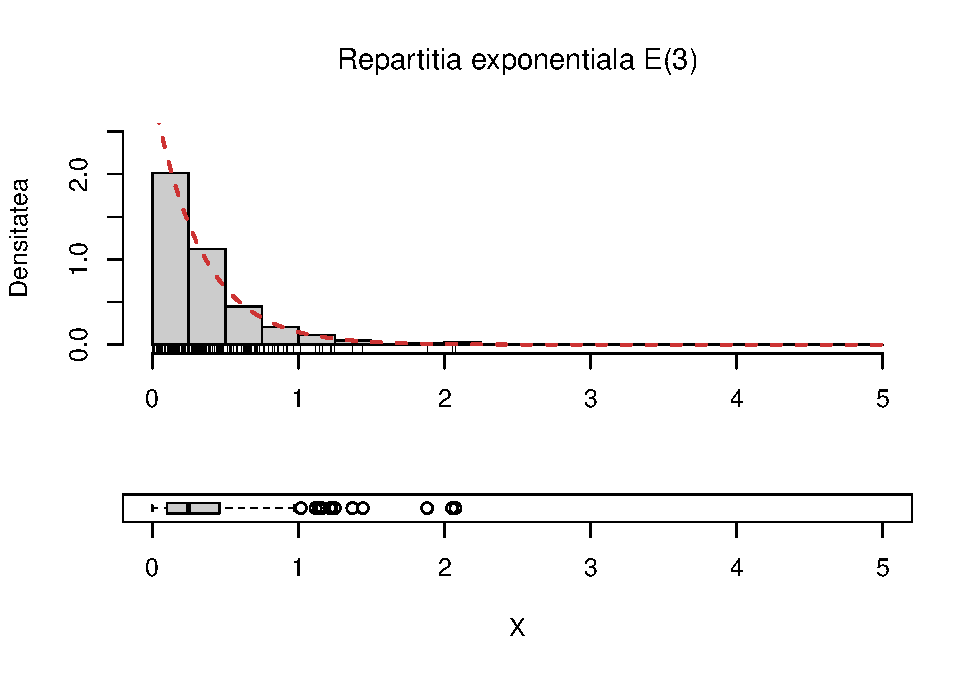
\includegraphics[width=0.7\linewidth]{Lab_6_files/figure-latex/unnamed-chunk-50-1} \end{center}

\section{Repartiția Cauchy}\label{repartitia-cauchy}

Spunem că o variabilă aleatoare \(X\) este repartizată \emph{Cauchy} de
parametrii \((0, 1)\), și se notează cu \(X\sim C(0,1)\), dacă
densitatea ei are forma

\[
  f_X(x) = \frac{1}{\pi} \frac{1}{1+x^2},\quad \forall x\in\mathbb{R}.
\]

Observăm că graficul densității repartiției Cauchy este asemănător cu
cel al repartiției normale. Parametrul \(M = 0\) reprezintă mediana (de
fapt \(\mathbb{P}(X\leq 0) = \mathbb{P}(X\geq 0) = \frac{1}{2}\))
variabilei aleatoare \(X\) și nu media iar prima și a treia cuartilă
sunt \(Q_1 = -1\) și respectiv \(Q_3=1\) (avem
\(\mathbb{P}(X\leq -1) = \mathbb{P}(X\geq 1) = \frac{1}{4}\)).

\begin{center}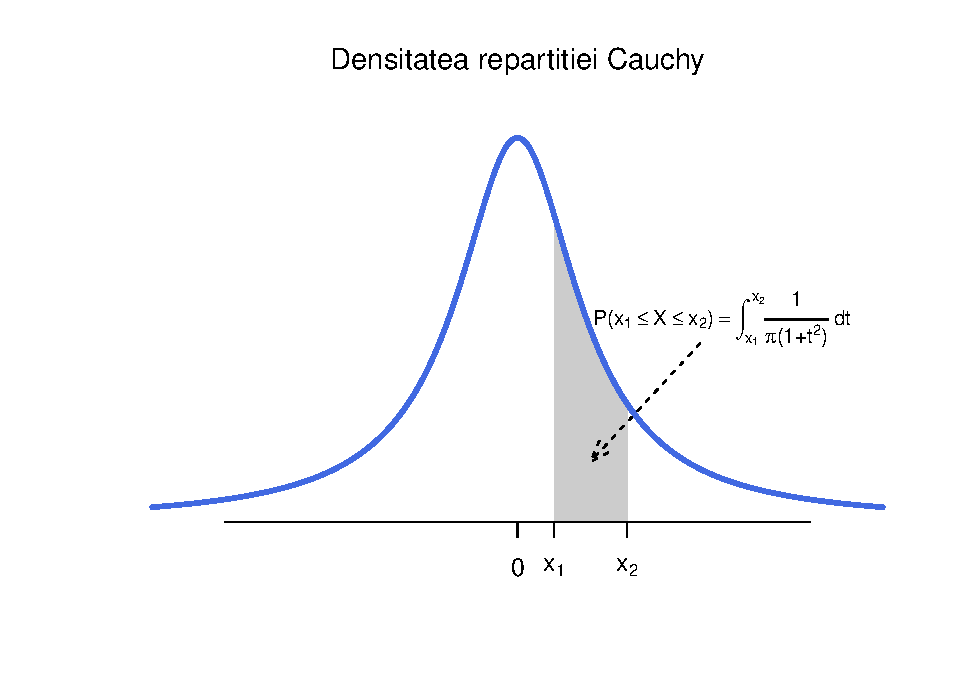
\includegraphics[width=0.7\linewidth]{Lab_6_files/figure-latex/unnamed-chunk-51-1} \end{center}

Funcția de repartiție a unei variabile aleatoare \(X\sim C(0,1)\) este
dată de

\[
  F_{X}(x) = \frac{1}{2} + \frac{1}{\pi}\arctan(x), \quad x\in \mathbb{R}.
\]

\begin{center}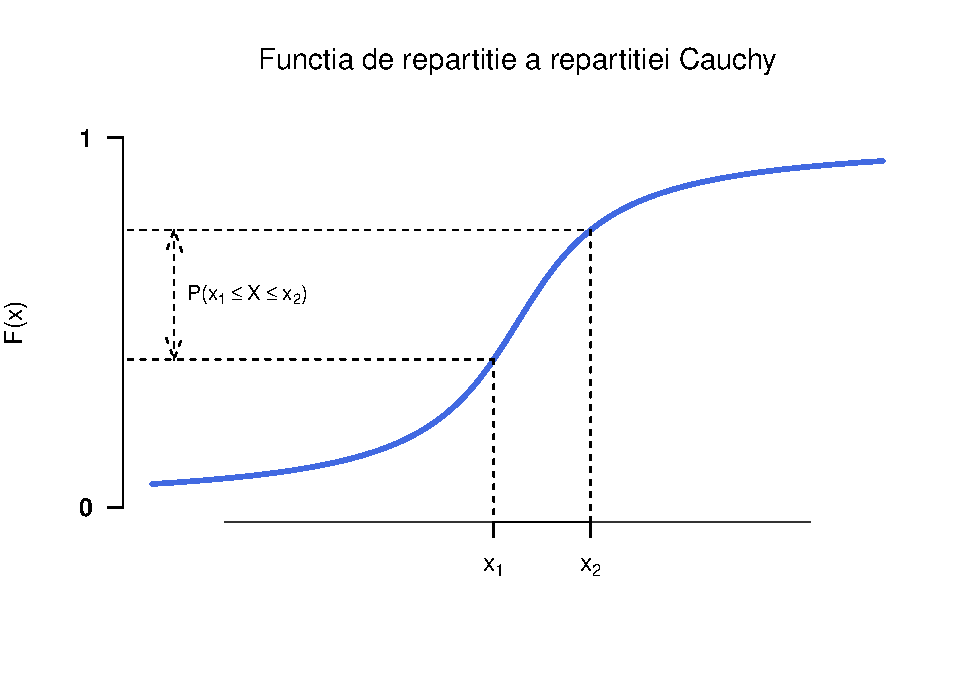
\includegraphics[width=0.7\linewidth]{Lab_6_files/figure-latex/unnamed-chunk-52-1} \end{center}

Media și varianța variabilei aleatoare \(X\sim C(0,1)\) \textbf{nu
există}.

\begin{rmdexercise}
Arătați că o variabilă aleatoare repartizată Cauchy \(C(0,1)\) nu are
medie.
\end{rmdexercise}

Fie \(Y\sim C(0,1)\) și \(\alpha, \beta\in\mathbb{R}\) cu \(\beta>0\).
Spunem că variabila aleatoare \(X = \alpha + \beta Y\) este repartizată
Cauchy de parametrii \((\alpha, \beta)\), \(X\sim C(\alpha, \beta)\).
Densitatea ei este

\[
  f_X(x) = \frac{1}{\pi\beta} \frac{1}{1+\left(\frac{x-\alpha}{\beta}\right)^2},\quad \forall x\in\mathbb{R}.
\]

Parametrii \(\alpha\) și \(\beta\) se interpretează în modul următor:
\(M = \alpha\) este mediana lui \(X\) iar \(Q_1 = \alpha-\beta\) și
\(Q_3 = \alpha + \beta\) reprezintă prima și a treia cuartilă.

În R putem să

\begin{itemize}
\tightlist
\item
  generăm observații independente din repartiția Cauchy
  \(C(\alpha, \beta)\) (e.g. \(\alpha = 0\), \(\beta = 2\))
\end{itemize}

\begin{Shaded}
\begin{Highlighting}[]
\KeywordTok{rcauchy}\NormalTok{(}\DecValTok{15}\NormalTok{, }\DataTypeTok{location =} \DecValTok{0}\NormalTok{, }\DataTypeTok{scale =} \DecValTok{2}\NormalTok{)}
\NormalTok{ [}\DecValTok{1}\NormalTok{] }\OperatorTok{-}\FloatTok{0.5966228}  \FloatTok{3.7627987}  \FloatTok{0.6864597} \OperatorTok{-}\FloatTok{0.4316018}  \FloatTok{1.4524446}  \FloatTok{0.3427032}
\NormalTok{ [}\DecValTok{7}\NormalTok{]  }\FloatTok{8.4285326}  \FloatTok{3.6056089}  \FloatTok{2.3506764} \OperatorTok{-}\FloatTok{3.5453329} \OperatorTok{-}\FloatTok{1.6137218} \FloatTok{10.4304800}
\NormalTok{[}\DecValTok{13}\NormalTok{] }\OperatorTok{-}\FloatTok{0.4449169}  \FloatTok{2.3005176} \OperatorTok{-}\FloatTok{3.6644199}
\end{Highlighting}
\end{Shaded}

\begin{itemize}
\tightlist
\item
  calculăm densitatea unei variabile aleatoare repartizate Cauchy
  \(C(\alpha, \beta)\) în diferite puncte
\end{itemize}

\begin{Shaded}
\begin{Highlighting}[]
\KeywordTok{dcauchy}\NormalTok{(}\KeywordTok{seq}\NormalTok{(}\OperatorTok{-}\DecValTok{5}\NormalTok{, }\DecValTok{5}\NormalTok{, }\DataTypeTok{length.out =} \DecValTok{20}\NormalTok{), }\DataTypeTok{location =} \DecValTok{1}\NormalTok{, }\DataTypeTok{scale =} \DecValTok{3}\NormalTok{)}
\NormalTok{ [}\DecValTok{1}\NormalTok{] }\FloatTok{0.02122066} \FloatTok{0.02450975} \FloatTok{0.02852541} \FloatTok{0.03345265} \FloatTok{0.03951056} \FloatTok{0.04693392}
\NormalTok{ [}\DecValTok{7}\NormalTok{] }\FloatTok{0.05591721} \FloatTok{0.06648594} \FloatTok{0.07825871} \FloatTok{0.09012539} \FloatTok{0.10006665} \FloatTok{0.10558334}
\NormalTok{[}\DecValTok{13}\NormalTok{] }\FloatTok{0.10494052} \FloatTok{0.09835367} \FloatTok{0.08782920} \FloatTok{0.07584810} \FloatTok{0.06425529} \FloatTok{0.05399054}
\NormalTok{[}\DecValTok{19}\NormalTok{] }\FloatTok{0.04532934} \FloatTok{0.03819719}
\end{Highlighting}
\end{Shaded}

\begin{itemize}
\tightlist
\item
  calculăm funcția de repartiție a unei variabile repartizate Cauchy
  \(C(\alpha, \beta)\) pentru diferite valori
\end{itemize}

\begin{Shaded}
\begin{Highlighting}[]
\KeywordTok{pcauchy}\NormalTok{(}\KeywordTok{seq}\NormalTok{(}\OperatorTok{-}\DecValTok{5}\NormalTok{, }\DecValTok{5}\NormalTok{, }\DataTypeTok{length.out =} \DecValTok{15}\NormalTok{), }\DataTypeTok{location =} \DecValTok{1}\NormalTok{, }\DataTypeTok{scale =} \DecValTok{3}\NormalTok{)}
\NormalTok{ [}\DecValTok{1}\NormalTok{] }\FloatTok{0.1475836} \FloatTok{0.1643213} \FloatTok{0.1848605} \FloatTok{0.2104166} \FloatTok{0.2425988} \FloatTok{0.2833834} \FloatTok{0.3347507}
\NormalTok{ [}\DecValTok{8}\NormalTok{] }\FloatTok{0.3975836} \FloatTok{0.4697759} \FloatTok{0.5451672} \FloatTok{0.6158581} \FloatTok{0.6764416} \FloatTok{0.7255627} \FloatTok{0.7644587}
\NormalTok{[}\DecValTok{15}\NormalTok{] }\FloatTok{0.7951672}
\end{Highlighting}
\end{Shaded}

\begin{itemize}
\tightlist
\item
  calculăm cuantilele de ordin \(p\in(0,1)\)
\end{itemize}

\begin{Shaded}
\begin{Highlighting}[]
\KeywordTok{qcauchy}\NormalTok{(}\KeywordTok{c}\NormalTok{(}\FloatTok{0.01}\NormalTok{, }\FloatTok{0.025}\NormalTok{, }\FloatTok{0.05}\NormalTok{, }\FloatTok{0.25}\NormalTok{, }\FloatTok{0.5}\NormalTok{, }\FloatTok{0.75}\NormalTok{, }\FloatTok{0.95}\NormalTok{, }\FloatTok{0.975}\NormalTok{, }\FloatTok{0.99}\NormalTok{), }\DataTypeTok{location =} \DecValTok{1}\NormalTok{, }\DataTypeTok{scale =} \DecValTok{3}\NormalTok{)}
\NormalTok{[}\DecValTok{1}\NormalTok{] }\OperatorTok{-}\FloatTok{94.46155} \OperatorTok{-}\FloatTok{37.11861} \OperatorTok{-}\FloatTok{17.94125}  \OperatorTok{-}\FloatTok{2.00000}   \FloatTok{1.00000}   \FloatTok{4.00000}  \FloatTok{19.94125}
\NormalTok{[}\DecValTok{8}\NormalTok{]  }\FloatTok{39.11861}  \FloatTok{96.46155}
\end{Highlighting}
\end{Shaded}

\begin{rmdexercise}
Generați \(2500\) de observații din repartiția Cauchy, trasați
histograma acestora și suprapuneți densitatea repartiției date pentru
intervalul \([-5,5]\) (vezi figura de mai jos).
\end{rmdexercise}

\begin{center}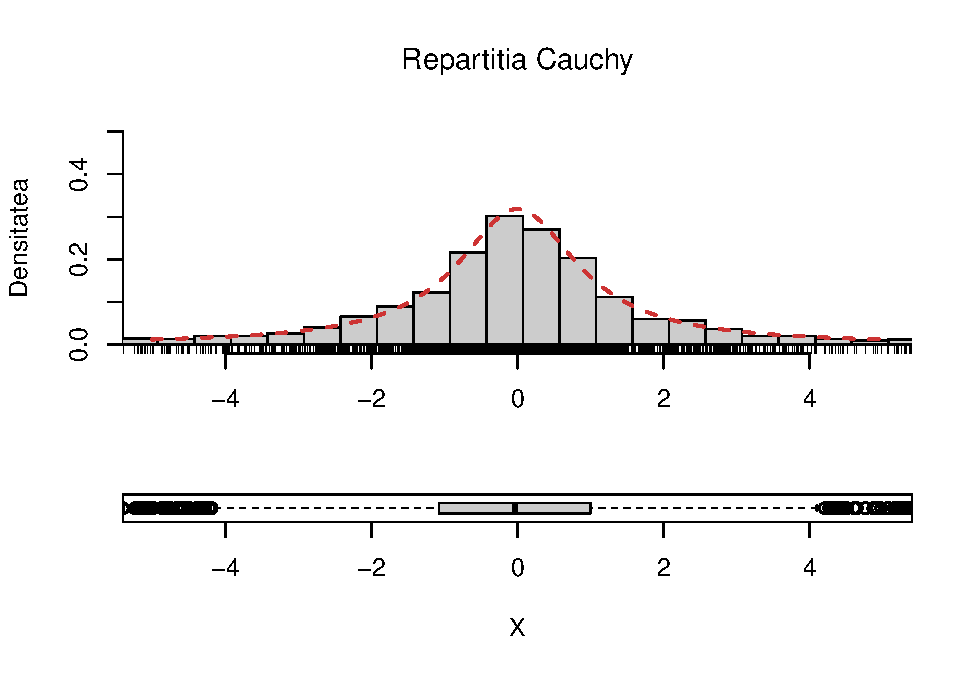
\includegraphics[width=0.7\linewidth]{Lab_6_files/figure-latex/unnamed-chunk-59-1} \end{center}

\begin{rmdexercise}
Fie \(X\) și \(Y\) două variabile aleatoare independente repartizate
\(\mathcal{N}(0,1)\). Arătați că variabila aleatoare \(\frac{X}{Y}\)
este repartizată Cauchy \(C(0,1)\).
\end{rmdexercise}

\begin{rmdexercise}
Fie \(X\) o variabilă aleatoare repartizată Cauchy \(C(\alpha, \beta)\).
Pentru fiecare pereche de parametrii \((\alpha, \beta)\) din mulțimea
\(\{(0,0.5), (0, 1), (0, 2), (-1, 1.5), (-2, 1)\}\) trasați pe același
grafic densitățile repartițiilor Cauchy cu parametrii
\((\alpha, \beta)\). Adăugați legendele corespunzătoare. Aceeași cerință
pentru funcțiile de repartiție.
\end{rmdexercise}

\begin{center}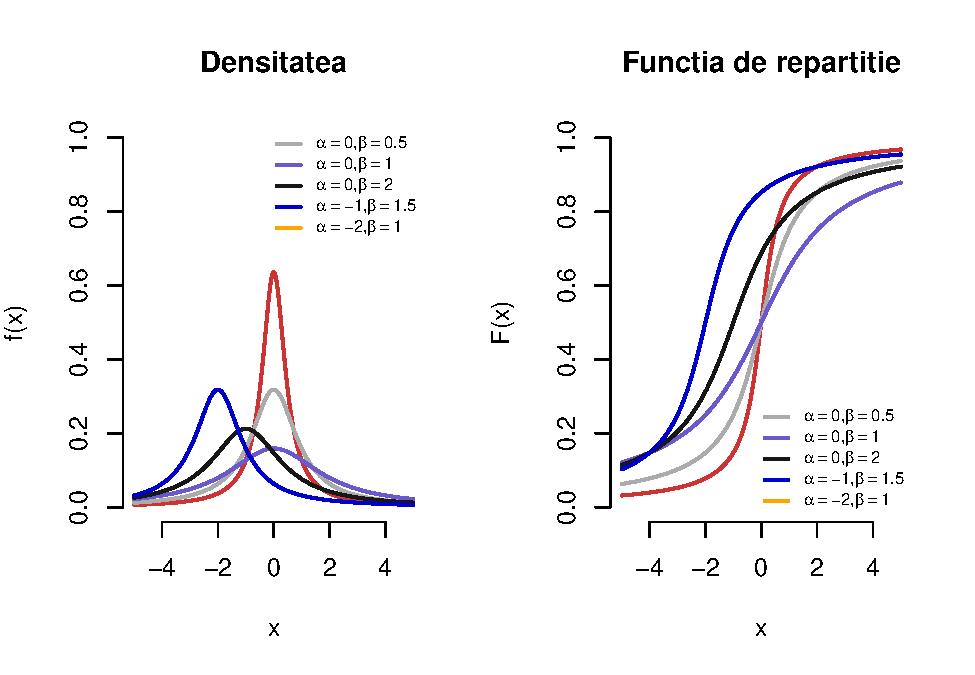
\includegraphics[width=0.7\linewidth]{Lab_6_files/figure-latex/unnamed-chunk-62-1} \end{center}

\begin{rmdexercise}
Folosind rezultatul de universalitate de la repartiția uniformă,
descrieți o procedură prin care puteți simula o variabilă aleatoare
repartizată Cauchy \(C(0,1)\) și construiți o funcție care permite
generarea de \(n\) observații independente dintr-o variabilă repartizată
\(X\sim C(\alpha, \beta)\). Verificați pentru parametrii \(\alpha = 3\)
și \(\beta = 5\) (a se vedea figura de mai jos).
\end{rmdexercise}

\begin{center}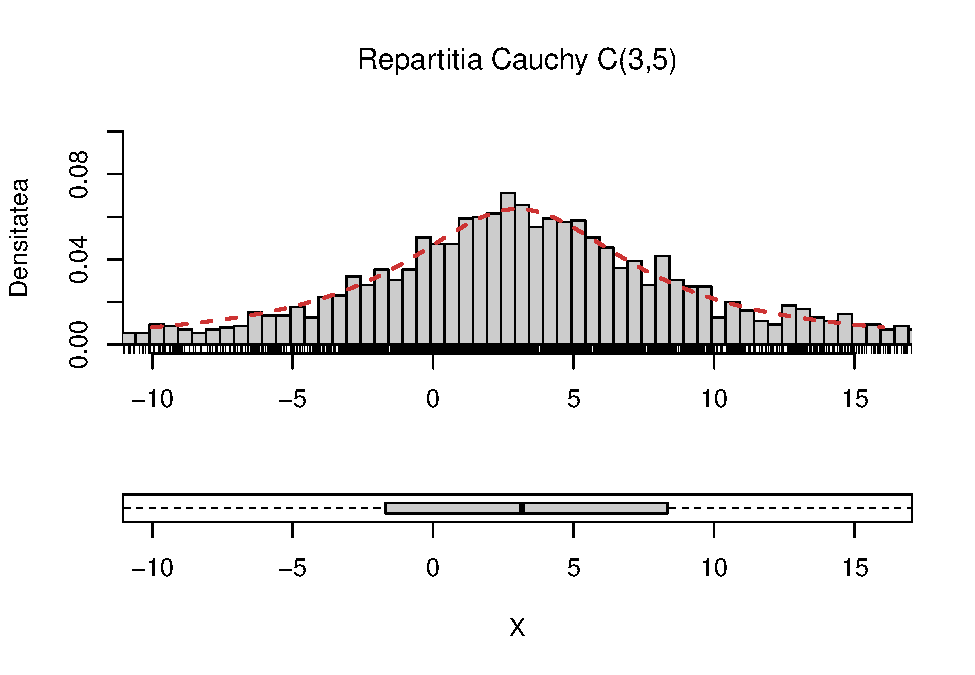
\includegraphics{Lab_6_files/figure-latex/unnamed-chunk-64-1} \end{center}

\section{Repartiția Gama}\label{repartitia-gama}

Spunem că o variabilă aleatoare \(X\) este repartizată \emph{Gama} de
parametrii \((\alpha, \beta)\), cu \(\alpha, \beta > 0\), și se notează
cu \(X\sim \Gamma(\alpha,\beta)\), dacă densitatea ei are forma

\[
  f_X(x) = \frac{\beta^{\alpha}}{\Gamma(\alpha)} x^{\alpha-1} e^{-\beta x},\quad \forall x>0.
\]

unde \(\Gamma(\alpha)\) este funcția (Gama, numită și integrală Euler de
al doilea tip) definită prin

\[
  \Gamma(\alpha) = \int_{0}^{\infty}x^{\alpha-1} e^{- x}\,dx,\quad \forall \alpha>0.
\]

\begin{center}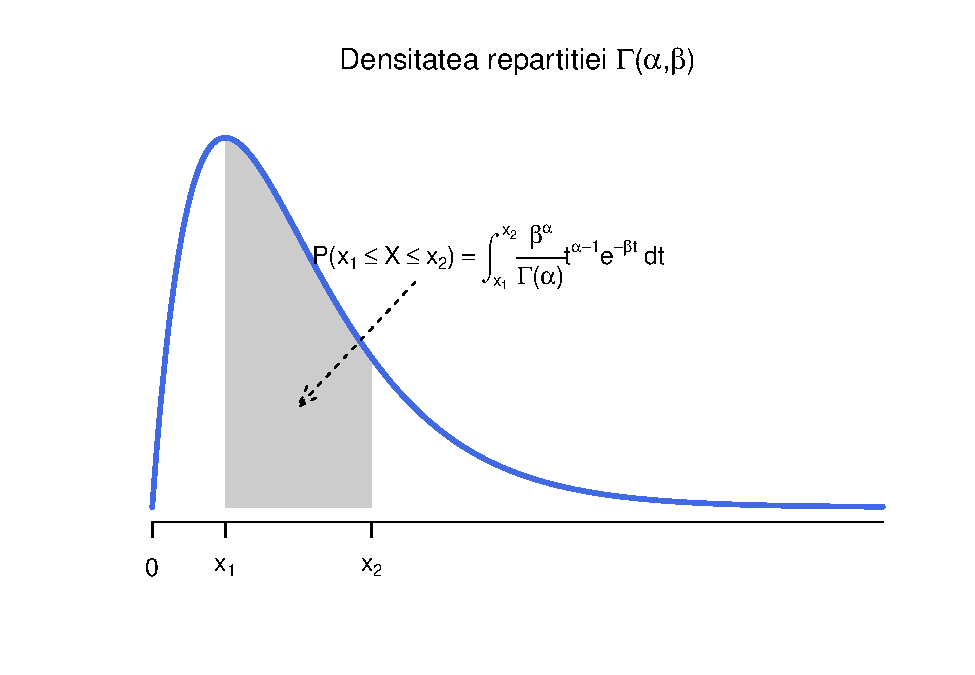
\includegraphics[width=0.7\linewidth]{Lab_6_files/figure-latex/unnamed-chunk-65-1} \end{center}

\begin{rmdexercise}
Arătați că funcția \(\Gamma(\alpha)\) verifică\footnote{Pentru mai multe
  proprietăți puteți consulta lucrarea lui E. Artin
  \href{http://plouffe.fr/simon/math/Artin\%20E.\%20The\%20Gamma\%20Function\%20(1931)(23s).pdf}{The
  Gamma Function}}:

\begin{enumerate}
\def\labelenumi{\arabic{enumi})}
\tightlist
\item
  \(\Gamma(1)=1\)
\item
  \(\Gamma(\alpha+1) = \alpha\Gamma(\alpha), \quad \forall \alpha>0\)
\item
  \(\Gamma(\alpha) = \beta^{\alpha}\int_{0}^{\infty}x^{\alpha-1} e^{- \beta x}\,dx,\quad \forall \alpha, \beta>0\)
\item
  \(\Gamma(n) = (n-1)!,\quad n = 1,2,\cdots\)
\item
  \(\Gamma(1/2) = \sqrt{\pi}\)
\end{enumerate}
\end{rmdexercise}

Funcția de repartiție a unei variabile aleatoare
\(X\sim \Gamma(\alpha, \beta)\) este dată de

\[
  F_{X}(x) = \int_{-\infty}^{x}f_X(t)\,dt = \frac{\beta^{\alpha}}{\Gamma(\alpha)}\int_{-\infty}^{x} t^{\alpha-1} e^{-\beta t}\,dt
\]

și nu are o formulă explicită de calcul.

\begin{center}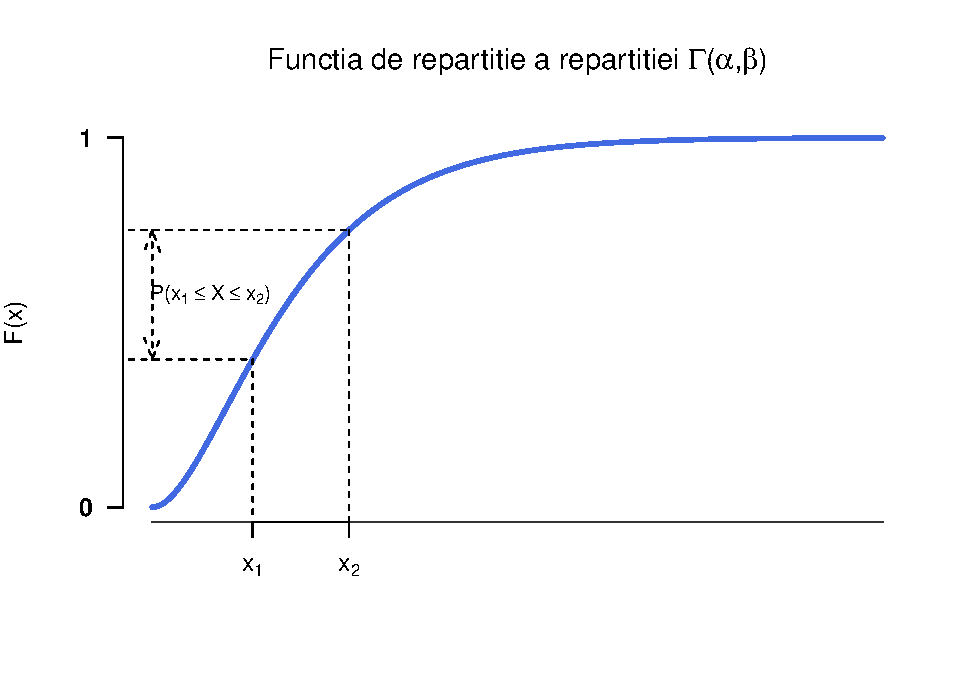
\includegraphics[width=0.7\linewidth]{Lab_6_files/figure-latex/unnamed-chunk-67-1} \end{center}

Observăm că repartiția \(\Gamma(1, \lambda)\) coincide cu repartiția
\(\mathcal{E}(\lambda)\).

Media și varianța variabilei aleatoare \(X\) repartizate Gama de
parametrii \(\Gamma(\alpha, \beta)\) sunt egale cu

\[
  \mathbb{E}[X] = \frac{\alpha}{\beta},\quad Var(X) = \frac{\alpha}{\beta^2}.
\]

\begin{rmdexercise}
Arătați că media și varianța unei variabile aleatoare repartizate Gama
de parametrii \(\alpha\) și \(\beta\) sunt egale cu

\[
  \mathbb{E}[X] = \frac{\alpha}{\beta},\quad Var(X) = \frac{\alpha}{\beta^2}. 
\]
\end{rmdexercise}

În R putem să

\begin{itemize}
\tightlist
\item
  generăm observații independente din repartiția
  \(\Gamma(\alpha, \beta)\) (e.g. \(\alpha = 2\), \(\beta = 2\))
\end{itemize}

\begin{Shaded}
\begin{Highlighting}[]
\KeywordTok{rgamma}\NormalTok{(}\DecValTok{15}\NormalTok{, }\DataTypeTok{shape =} \DecValTok{2}\NormalTok{, }\DataTypeTok{rate =} \DecValTok{2}\NormalTok{)}
\NormalTok{ [}\DecValTok{1}\NormalTok{] }\FloatTok{0.2739606} \FloatTok{1.0172288} \FloatTok{1.6546379} \FloatTok{0.4210210} \FloatTok{0.8476985} \FloatTok{0.2928765} \FloatTok{0.6798413}
\NormalTok{ [}\DecValTok{8}\NormalTok{] }\FloatTok{1.1393160} \FloatTok{1.0763898} \FloatTok{1.4411221} \FloatTok{0.9500644} \FloatTok{0.7387296} \FloatTok{0.4159926} \FloatTok{0.8942659}
\NormalTok{[}\DecValTok{15}\NormalTok{] }\FloatTok{0.8366199}
\end{Highlighting}
\end{Shaded}

\begin{itemize}
\tightlist
\item
  calculăm densitatea unei variabile aleatoare repartizate
  \(\Gamma(\alpha, \beta)\) în diferite puncte
\end{itemize}

\begin{Shaded}
\begin{Highlighting}[]
\KeywordTok{dgamma}\NormalTok{(}\KeywordTok{seq}\NormalTok{(}\DecValTok{0}\NormalTok{, }\DecValTok{5}\NormalTok{, }\DataTypeTok{length.out =} \DecValTok{20}\NormalTok{), }\DataTypeTok{shape =} \DecValTok{1}\NormalTok{, }\DataTypeTok{rate =} \DecValTok{3}\NormalTok{)}
\NormalTok{ [}\DecValTok{1}\NormalTok{] }\FloatTok{3.000000e+00} \FloatTok{1.362251e+00} \FloatTok{6.185761e-01} \FloatTok{2.808853e-01} \FloatTok{1.275455e-01}
\NormalTok{ [}\DecValTok{6}\NormalTok{] }\FloatTok{5.791632e-02} \FloatTok{2.629886e-02} \FloatTok{1.194188e-02} \FloatTok{5.422615e-03} \FloatTok{2.462321e-03}
\NormalTok{[}\DecValTok{11}\NormalTok{] }\FloatTok{1.118100e-03} \FloatTok{5.077110e-04} \FloatTok{2.305433e-04} \FloatTok{1.046860e-04} \FloatTok{4.753619e-05}
\NormalTok{[}\DecValTok{16}\NormalTok{] }\FloatTok{2.158541e-05} \FloatTok{9.801583e-06} \FloatTok{4.450739e-06} \FloatTok{2.021008e-06} \FloatTok{9.177070e-07}
\end{Highlighting}
\end{Shaded}

\begin{itemize}
\tightlist
\item
  calculăm funcția de repartiție a unei variabile repartizate
  \(\Gamma(\alpha, \beta)\) pentru diferite valori
\end{itemize}

\begin{Shaded}
\begin{Highlighting}[]
\KeywordTok{pgamma}\NormalTok{(}\KeywordTok{seq}\NormalTok{(}\DecValTok{0}\NormalTok{, }\DecValTok{5}\NormalTok{, }\DataTypeTok{length.out =} \DecValTok{15}\NormalTok{), }\DataTypeTok{shape =} \DecValTok{1}\NormalTok{, }\DataTypeTok{rate =} \DecValTok{3}\NormalTok{)}
\NormalTok{ [}\DecValTok{1}\NormalTok{] }\FloatTok{0.0000000} \FloatTok{0.6574811} \FloatTok{0.8826808} \FloatTok{0.9598160} \FloatTok{0.9862362} \FloatTok{0.9952856} \FloatTok{0.9983852}
\NormalTok{ [}\DecValTok{8}\NormalTok{] }\FloatTok{0.9994469} \FloatTok{0.9998106} \FloatTok{0.9999351} \FloatTok{0.9999778} \FloatTok{0.9999924} \FloatTok{0.9999974} \FloatTok{0.9999991}
\NormalTok{[}\DecValTok{15}\NormalTok{] }\FloatTok{0.9999997}
\end{Highlighting}
\end{Shaded}

\begin{itemize}
\tightlist
\item
  calculăm cuantilele de ordin \(p\in(0,1)\)
\end{itemize}

\begin{Shaded}
\begin{Highlighting}[]
\KeywordTok{qgamma}\NormalTok{(}\KeywordTok{c}\NormalTok{(}\FloatTok{0.01}\NormalTok{, }\FloatTok{0.025}\NormalTok{, }\FloatTok{0.05}\NormalTok{, }\FloatTok{0.25}\NormalTok{, }\FloatTok{0.5}\NormalTok{, }\FloatTok{0.75}\NormalTok{, }\FloatTok{0.95}\NormalTok{, }\FloatTok{0.975}\NormalTok{, }\FloatTok{0.99}\NormalTok{), }\DataTypeTok{shape =} \DecValTok{1}\NormalTok{, }\DataTypeTok{rate =} \DecValTok{3}\NormalTok{)}
\NormalTok{[}\DecValTok{1}\NormalTok{] }\FloatTok{0.003350112} \FloatTok{0.008439269} \FloatTok{0.017097765} \FloatTok{0.095894024} \FloatTok{0.231049060} \FloatTok{0.462098120}
\NormalTok{[}\DecValTok{7}\NormalTok{] }\FloatTok{0.998577425} \FloatTok{1.229626485} \FloatTok{1.535056729}
\end{Highlighting}
\end{Shaded}

\begin{rmdexercise}
Fie \(X\) o variabilă aleatoare repartizată \(\Gamma(\alpha, \beta)\).
Pentru fiecare pereche de parametrii \((\alpha, \beta)\) din mulțimea
\(\{(1,0.5), (2, 0.5), (3, 0.5), (5, 1), (9, 0.5), (7.5, 1), (0.5, 1) \}\)
trasați pe același grafic densitățile repartițiilor Gama cu parametrii
\((\alpha, \beta)\). Adăugați legendele corespunzătoare. Aceeași cerință
pentru funcțiile de repartiție.
\end{rmdexercise}

\begin{center}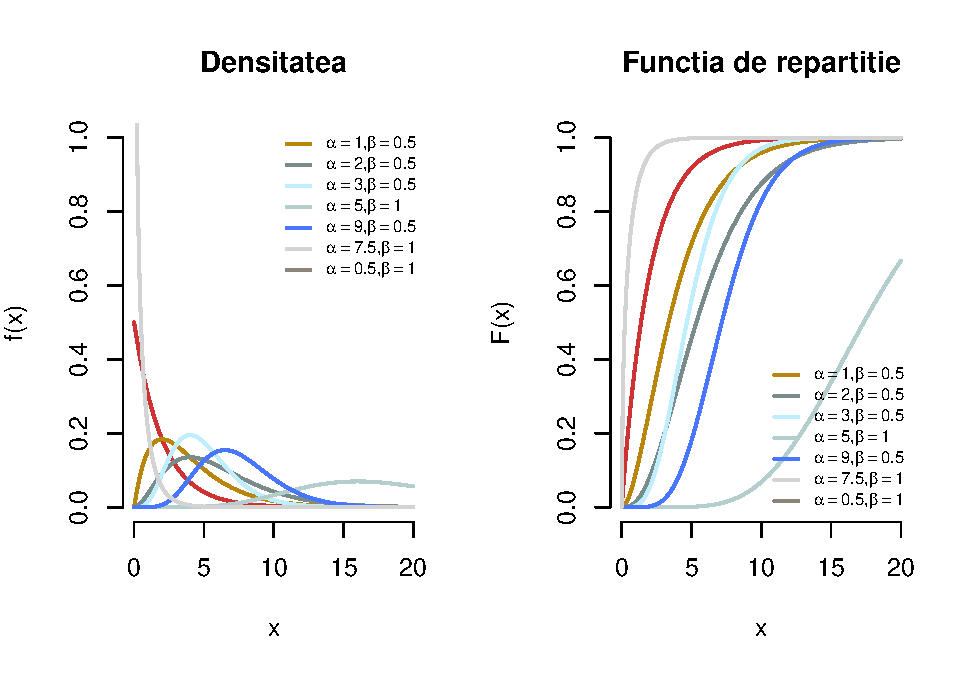
\includegraphics[width=0.7\linewidth]{Lab_6_files/figure-latex/unnamed-chunk-74-1} \end{center}

\begin{rmdexercise}
Generați \(250\) de observații din repartiția \(\Gamma(9,2)\), trasați
histograma acestora și suprapuneți densitatea repartiției date (vezi
figura de mai jos).
\end{rmdexercise}

\begin{center}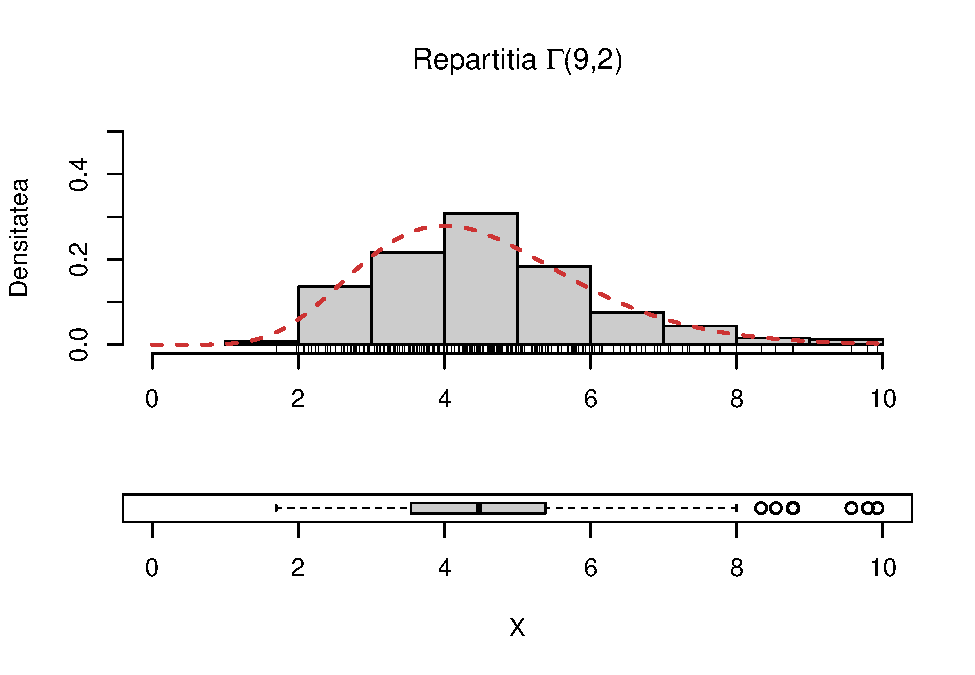
\includegraphics[width=0.7\linewidth]{Lab_6_files/figure-latex/unnamed-chunk-76-1} \end{center}

\section{Repartiția Beta}\label{repartitia-beta}

Spunem că o variabilă aleatoare \(X\) este repartizată \emph{Beta} de
parametrii \((\alpha, \beta)\), cu \(\alpha, \beta > 0\), și se notează
cu \(X\sim B(\alpha,\beta)\), dacă densitatea ei are forma

\[
  f_X(x) = \frac{1}{B(\alpha, \beta)} x^{\alpha-1} (1-x)^{\beta-1},\quad 0\leq x\leq 1.
\] unde \(B(\alpha, \beta)\) este funcția (Beta, numită și integrală
Euler de primul tip) definită prin

\[
  B(\alpha, \beta) = \int_{0}^{\infty}x^{\alpha-1} (1-x)^{\beta-1}\,dx,\quad \forall \alpha, \beta >0.
\]

\begin{center}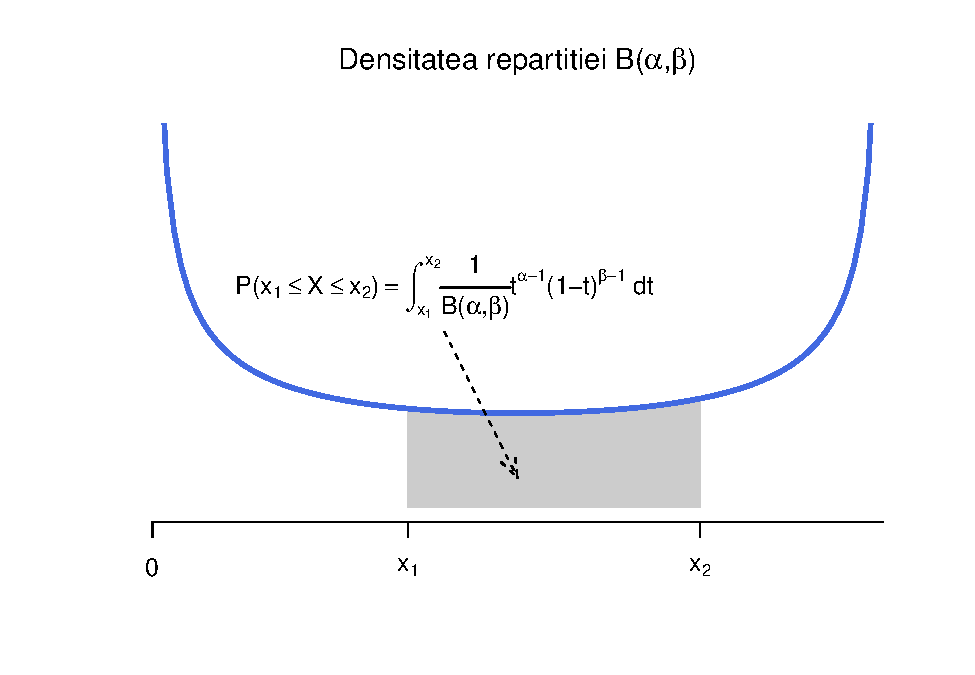
\includegraphics[width=0.7\linewidth]{Lab_6_files/figure-latex/unnamed-chunk-77-1} \end{center}

\begin{rmdexercise}
Arătați că funcția Beta \(B(\alpha, \beta)\) verifică următoarele
proprietăți:

\begin{enumerate}
\def\labelenumi{\arabic{enumi})}
\tightlist
\item
  \(B(\alpha, \beta) = \frac{\Gamma(\alpha)\Gamma(\beta)}{\Gamma(\alpha+\beta)}\)
\item
  \(B(\alpha, \beta) = B(\beta, \alpha)\)
\item
  \(B(\alpha, \beta) = B(\alpha, \beta+1) + B(\alpha+1, \beta)\)
\item
  \(B(\alpha + 1, \beta) = B(\alpha, \beta) \frac{\alpha}{\alpha+\beta}\)
  și
  \(B(\alpha, \beta + 1) = B(\alpha, \beta) \frac{\beta}{\alpha+\beta}\).
\end{enumerate}
\end{rmdexercise}

Funcția de repartiție a unei variabile aleatoare
\(X\sim B(\alpha, \beta)\) este dată de

\[
  F_{X}(x) = \int_{-\infty}^{x}f_X(t)\,dt = \frac{1}{B(\alpha, \beta)} \int_{-\infty}^{x} t^{\alpha-1} (1-t)^{\beta-1}\,dt
\]

și nu are o formulă explicită de calcul.

\begin{center}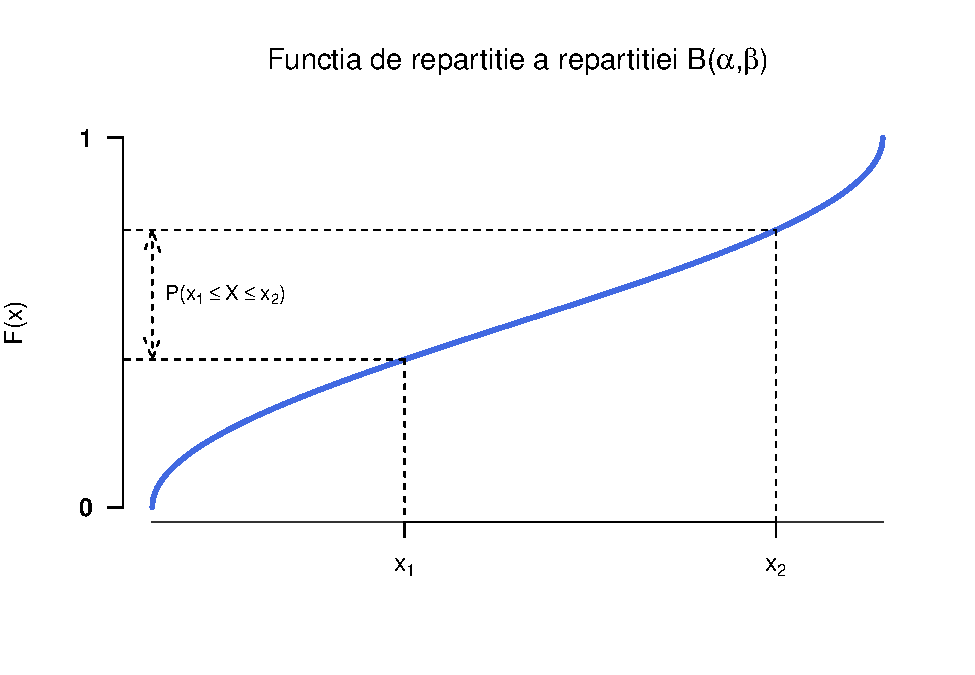
\includegraphics[width=0.7\linewidth]{Lab_6_files/figure-latex/unnamed-chunk-79-1} \end{center}

Observăm că repartiția \(B(1, 1)\) coincide cu repartiția
\(\mathcal{U}([0,1])\).

Media și varianța variabilei aleatoare \(X\) repartizate Gamma de
parametrii \(B(\alpha, \beta)\) sunt egale cu

\[
  \mathbb{E}[X] = \frac{\alpha}{\alpha+\beta},\quad Var(X) = \frac{\alpha\beta}{(\alpha+\beta)^2(\alpha+\beta+1)}.
\]

Observăm că \(Var(X)\leq\mathbb{E}[X](1-\mathbb{E}[X])\).

\begin{rmdexercise}
Arătați că media și varianța unei variabile aleatoare repartizate Beta
de parametrii \(\alpha\) și \(\beta\) sunt egale cu

\[
  \mathbb{E}[X] = \frac{\alpha}{\alpha+\beta},\quad Var(X) = \frac{\alpha\beta}{(\alpha+\beta)^2(\alpha+\beta+1)}. 
\]
\end{rmdexercise}

În R putem să

\begin{itemize}
\tightlist
\item
  generăm observații independente din repartiția \(B(\alpha, \beta)\)
  (e.g. \(\alpha = 2.5\), \(\beta = 1\))
\end{itemize}

\begin{Shaded}
\begin{Highlighting}[]
\KeywordTok{rbeta}\NormalTok{(}\DecValTok{15}\NormalTok{, }\DataTypeTok{shape1 =} \FloatTok{2.5}\NormalTok{, }\DataTypeTok{shape2 =} \DecValTok{1}\NormalTok{)}
\NormalTok{ [}\DecValTok{1}\NormalTok{] }\FloatTok{0.7945436} \FloatTok{0.7609136} \FloatTok{0.9265073} \FloatTok{0.9309420} \FloatTok{0.5621874} \FloatTok{0.3664261} \FloatTok{0.9694945}
\NormalTok{ [}\DecValTok{8}\NormalTok{] }\FloatTok{0.5804873} \FloatTok{0.9504669} \FloatTok{0.9115169} \FloatTok{0.8457509} \FloatTok{0.6717780} \FloatTok{0.7213322} \FloatTok{0.9738473}
\NormalTok{[}\DecValTok{15}\NormalTok{] }\FloatTok{0.9791769}
\end{Highlighting}
\end{Shaded}

\begin{itemize}
\tightlist
\item
  calculăm densitatea unei variabile aleatoare repartizate
  \(B(\alpha, \beta)\) în diferite puncte
\end{itemize}

\begin{Shaded}
\begin{Highlighting}[]
\KeywordTok{dbeta}\NormalTok{(}\KeywordTok{seq}\NormalTok{(}\DecValTok{0}\NormalTok{, }\DecValTok{1}\NormalTok{, }\DataTypeTok{length.out =} \DecValTok{20}\NormalTok{), }\DataTypeTok{shape1 =} \DecValTok{1}\NormalTok{, }\DataTypeTok{shape2 =} \DecValTok{3}\NormalTok{)}
\NormalTok{ [}\DecValTok{1}\NormalTok{] }\FloatTok{3.000000000} \FloatTok{2.692520776} \FloatTok{2.401662050} \FloatTok{2.127423823} \FloatTok{1.869806094}
\NormalTok{ [}\DecValTok{6}\NormalTok{] }\FloatTok{1.628808864} \FloatTok{1.404432133} \FloatTok{1.196675900} \FloatTok{1.005540166} \FloatTok{0.831024931}
\NormalTok{[}\DecValTok{11}\NormalTok{] }\FloatTok{0.673130194} \FloatTok{0.531855956} \FloatTok{0.407202216} \FloatTok{0.299168975} \FloatTok{0.207756233}
\NormalTok{[}\DecValTok{16}\NormalTok{] }\FloatTok{0.132963989} \FloatTok{0.074792244} \FloatTok{0.033240997} \FloatTok{0.008310249} \FloatTok{0.000000000}
\end{Highlighting}
\end{Shaded}

\begin{itemize}
\tightlist
\item
  calculăm funcția de repartiție a unei variabile repartizate
  \(B(\alpha, \beta)\) pentru diferite valori
\end{itemize}

\begin{Shaded}
\begin{Highlighting}[]
\KeywordTok{pbeta}\NormalTok{(}\KeywordTok{seq}\NormalTok{(}\DecValTok{0}\NormalTok{, }\DecValTok{1}\NormalTok{, }\DataTypeTok{length.out =} \DecValTok{15}\NormalTok{), }\DataTypeTok{shape1 =} \DecValTok{1}\NormalTok{, }\DataTypeTok{shape2 =} \DecValTok{3}\NormalTok{)}
\NormalTok{ [}\DecValTok{1}\NormalTok{] }\FloatTok{0.0000000} \FloatTok{0.1993440} \FloatTok{0.3702624} \FloatTok{0.5149417} \FloatTok{0.6355685} \FloatTok{0.7343294} \FloatTok{0.8134111}
\NormalTok{ [}\DecValTok{8}\NormalTok{] }\FloatTok{0.8750000} \FloatTok{0.9212828} \FloatTok{0.9544461} \FloatTok{0.9766764} \FloatTok{0.9901603} \FloatTok{0.9970845} \FloatTok{0.9996356}
\NormalTok{[}\DecValTok{15}\NormalTok{] }\FloatTok{1.0000000}
\end{Highlighting}
\end{Shaded}

\begin{itemize}
\tightlist
\item
  calculăm cuantilele de ordin \(p\in(0,1)\)
\end{itemize}

\begin{Shaded}
\begin{Highlighting}[]
\KeywordTok{qbeta}\NormalTok{(}\KeywordTok{c}\NormalTok{(}\FloatTok{0.01}\NormalTok{, }\FloatTok{0.025}\NormalTok{, }\FloatTok{0.05}\NormalTok{, }\FloatTok{0.25}\NormalTok{, }\FloatTok{0.5}\NormalTok{, }\FloatTok{0.75}\NormalTok{, }\FloatTok{0.95}\NormalTok{, }\FloatTok{0.975}\NormalTok{, }\FloatTok{0.99}\NormalTok{), }\DataTypeTok{shape1 =} \DecValTok{1}\NormalTok{, }\DataTypeTok{shape2 =} \DecValTok{3}\NormalTok{)}
\NormalTok{[}\DecValTok{1}\NormalTok{] }\FloatTok{0.003344507} \FloatTok{0.008403759} \FloatTok{0.016952428} \FloatTok{0.091439704} \FloatTok{0.206299474} \FloatTok{0.370039475}
\NormalTok{[}\DecValTok{7}\NormalTok{] }\FloatTok{0.631596850} \FloatTok{0.707598226} \FloatTok{0.784556531}
\end{Highlighting}
\end{Shaded}

\begin{rmdexercise}
Fie \(X\) o variabilă aleatoare repartizată \(B(\alpha, \beta)\). Pentru
fiecare pereche de parametrii \((\alpha, \beta)\) din mulțimea
\(\{(0.5,0.5), (1, 3), (5, 1), (2, 2), (2, 5)\}\) trasați pe același
grafic densitățile repartițiilor Beta cu parametrii \((\alpha, \beta)\).
Adăugați legendele corespunzătoare. Aceeași cerință pentru funcțiile de
repartiție.
\end{rmdexercise}

\begin{center}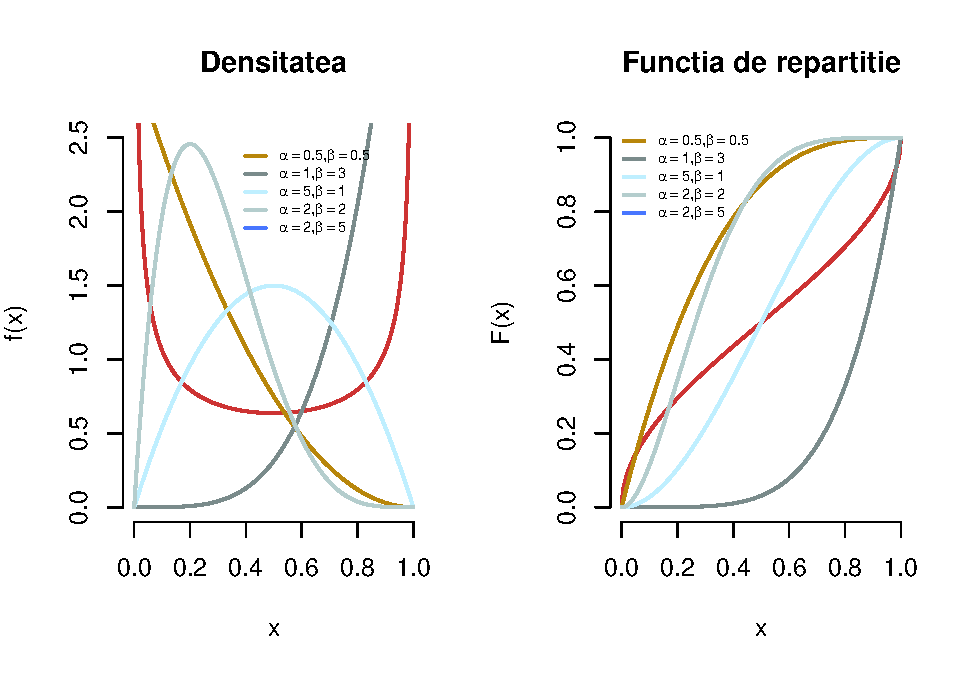
\includegraphics[width=0.7\linewidth]{Lab_6_files/figure-latex/unnamed-chunk-86-1} \end{center}

\begin{rmdexercise}
Generați \(250\) de observații din repartiția \(B(3,3)\), trasați
histograma acestora și suprapuneți densitatea repartiției date (vezi
figura de mai jos).
\end{rmdexercise}

\begin{center}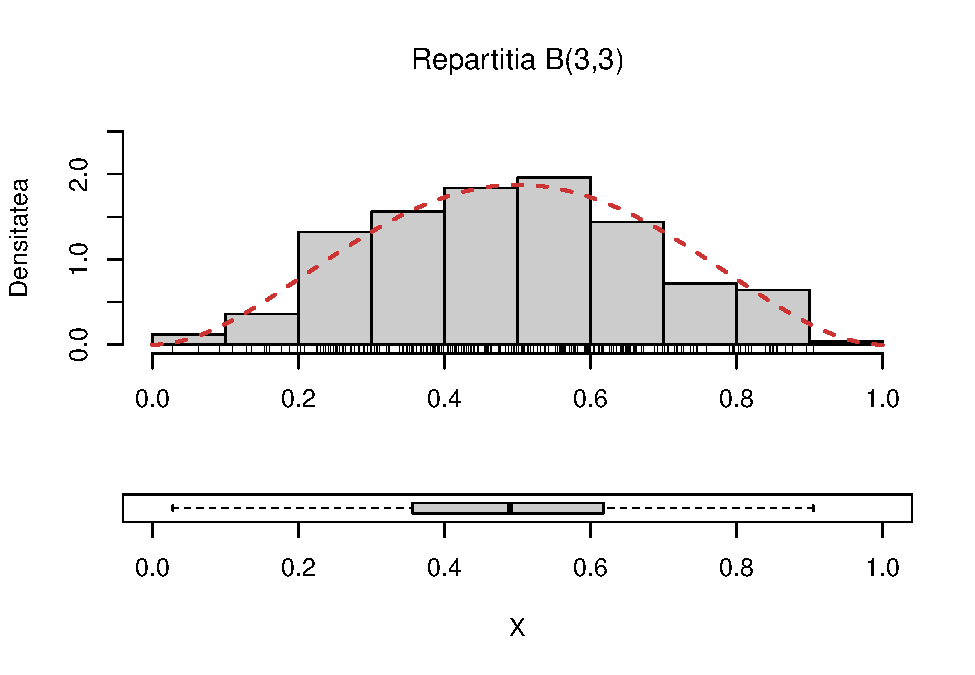
\includegraphics[width=0.7\linewidth]{Lab_6_files/figure-latex/unnamed-chunk-88-1} \end{center}


\end{document}
